% !TeX encoding = UTF-8
% !TeX spellcheck = en_GB
% !TeX root = ../thesis.tex

\chapter{Architecture/System Design}
\label{chapter:design}

The REPUSH (Reconfigurable PUF against Session Hijacking) protocol is designed to address a fundamental flaw in current session security: the absence of trusted continuous authentication after the initial login event. Existing continuous session validation approaches totally trust the host machine to faithfully mediate all interactions between the user and the server. In practice, the main attack vector for session hijacking is cookie theft. Such theft is carried out through specialized malware, so called "Infostealers", which the victim runs on their machine through some elaborate social engineering trick. 

The main observation motivating REPUSH is as follows: if the "Infostealer" malware has remote code execution abilities, which is a prerequisite for cookie theft, then it follows that this same malware could be adapted to further exploit any kind of continuous session validation scheme that the user is using. To give an example with the previously presented PUSH protocol, any malware could in theory use the dongle to sign cookies and silently prove ownership of the dongle. The host computer's role as a trusted intermediary is what makes this attack possible. 

REPUSH eliminates this attack surface by assuming that the host is potentially compromised. Similar to PUSH, REPUSH uses an external dongle as proof of ownership of a session. Under this new threat model, the dongle must be adapted so that the compromised host does not exploit it. Another key improvement is the use of an LR-PUF to augment a weak PUF for fast ephemeral key generation. In this chapter, we will explore the design goals and security requirements that motivate the REPUSH protocol, define the threat model and assumptions under which the protocol operates, introduce the protocol parties and their respective roles, define each phase of the protocol in detail, and describe the logical design of the dongle. In doing so, this chapter addresses research question 1 by redesigning the PUSH protocol around a fully compromised host threat model, and it addresses research question 2 by explaining how the LR-PUF's reconfiguration property is integrated into the protocol.  

\section{Design Goals and Security Requirements}
Balancing between security and usability is a delicate act that requires careful design. REPUSH is driven by two goals: security goals which define the threats that the protocol must protect against, and usability goals which ensure user-friendliness and that the protocol remains practical for deployment. 

\subsection{Security Goals}

The protocol's primary security requirement is continuous session authentication: a session token or cookie obtained by the attacker should be insufficient to own the session. Rather, ownership of the dongle must be demonstrated at specified intervals, and sensitive requests must be signed by the dongle after explicit approval by the user on the dongle's user interface. 

Since the host computer is not trusted, all cryptographic operations such as signing and encryption, key storage, and user approval should occur exclusively within the dongle which will act as an isolated trusted computing environment. Furthermore, the protocol is designed according to the least privilege principle, which means that each party only holds the data it needs to carry out its role in the protocol. 

The protocol should also provide mutual authentication, i.e. the dongle must verify the server's identity, and the server must verify that the dongle does belong to some user. 

Since sensitive requests must be approved on the dongle's own user interface, the user has full transparency on the requests they make to the server. A compromised host cannot compromise the dongle, as in even if it were to make a request to it, the dongle will clearly and transparently show what that request is on its screen. This trusted display concept \cite{ledgertrusteddisplay} is similar to how some cryptocurrency physical wallets have a screen which shows which receiving address will receive the cryptocurrency to avoid sending it to another address in case the user's computer is compromised (see figure \ref{fig:trusted-display}). 

As a further consequence of this user intent confirmation on a trusted display, we get passive compromise detection. Because every sensitive request must be approved by the user on the dongle's screen, any attempt by malware to invoke a signing operation for a sensitive request will immediately alert the user, as they would see a request they did not intend. This acts as a way to detect intrusion and then independently take the necessary precautions and steps to remediate it. Unlike traditional intrusion detection systems running on the host, the dongle provides a reliable intrusion indicator of compromise that even the most privileged of malware cannot bypass.

\begin{figure}[ht!]
    \centering
    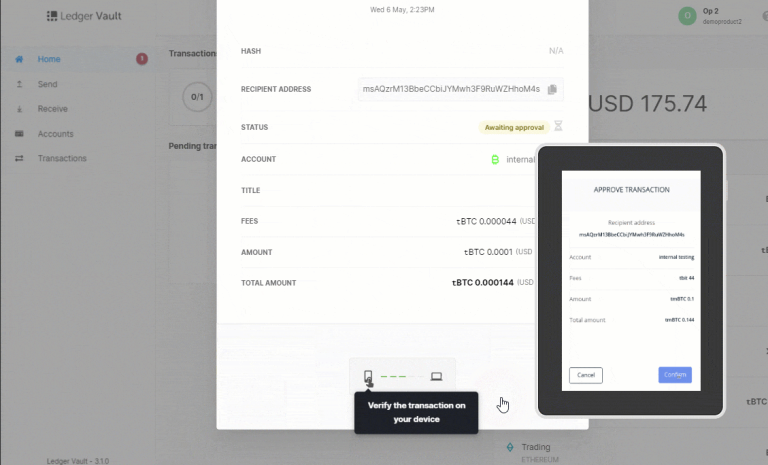
\includegraphics[width=0.8\textwidth]{img/ledger.png}
    \caption{Trusted display on Ledger wallet to confirm a transaction. \cite{ledgertrusteddisplay}}
    \label{fig:trusted-display}
\end{figure} 

\subsection{Usability Goals}
Security mechanisms that produce excessive friction are circumvented or disabled by users. The security goals must therefore be supplemented with usability goals to reduce friction. To this end, the protocol distinguishes between high risk sensitive and low risk non-sensitive requests. Similar to standard requests in PUSH, non-sensitive requests are processed and accepted by the server without any user interaction within a validity window $T_{Validity}$ which will be explained in more detail in the protocol design section. On the other hand, sensitive requests require explicit approval on the dongle's touch screen. In general, sensitive requests are less frequent compared to non-sensitive ones, hence there should be no noticeable friction as users are already familiar with the friction introduced by MFA in some cases. This selective friction concept ensures that only sensitive operations that warrant scrutiny should burden the user. 

When dongle interaction is required, the presented information on the display must be succinct enough to allow the user to make a quick informed decision. This reduces cognitive load and limits room for confusion or error. 

The latency introduced by the protocol should be minimal and unnoticeable.

Finally, the adoption of the REPUSH protocol should not require significant modifications to existing web applications. When possible established and familiar concepts and protocols are used.

\section{Threat Model and Assumptions}
REPUSH was designed with a concrete threat model that specifies a potential attacker's capabilities, and with assumptions about each of the protocol parties. 

\subsection{Attacker Model}
The attacker is assumed to have arbitrary code execution abilities on the host. This includes the ability to read and write any memory accessible to the browser or the dongle manager processes, and the ability to intercept and tamper with the inter-process communication, make requests on behalf of the user, and exfiltrate session cookies. Furthermore, the network channel between the host and the server is likewise treated as under the control of the adversary.

In contrast, the attacker is assumed to be incapable of physically interacting with the dongle, any attack requiring physical access to the dongle is therefore outside the scope of this protocol. Moreover, the attacker is assumed to be computationally bounded and unable to break the used signature and encryption schemes within any reasonable time frame.

\subsection{Trust Assumptions}
The REPUSH protocol operates under the assumption that the dongle and the server are the sole fully trusted parties. Everything else on the machine including the browser and the dongle manager (DOMAN) is treated as untrusted as they could be potentially under the control of the attacker in case of a malware infection. The user is assumed to be cooperative and aware enough to read and respond to the prompts presented on the dongle. 

\section{Protocol Parties}
REPUSH involves the following five parties:
\subsection{The Dongle}
The dongle is an external hardware device in the user's possession and the sole trusted party along the server. It serves as the protocol's root of trust, performing all security critical operations in isolation from the host. The dongle consists of an LR-PUF, a processing unit, and a touch screen, and connects to the host via USB. The dongle is responsible for the following:
\begin{itemize}
    \item Storing the CA's public key to authenticate servers.
    \item Generating ephemeral asymmetric key pairs using an LR-PUF construction and never exposing the generated private keys.
    \item Signing and encrypting payloads sent by the host according to the protocol specifications to prove ownership of the dongle.
    \item Prompting the user to accept or deny the signing of sensitive requests.
    \item Authenticating the user with the server by taking the user's login credentials (username and password) via user input on the touch screen or optionally by acting as a password manager.
\end{itemize}

\subsection{The Dongle Manager (DOMAN)}
DOMAN (Dongle Manager) is a local HTTP server on the host that acts as a middleman between the browser and the dongle. Since the browser typically cannot control serial devices, DOMAN exposes an HTTP API that the browser calls via JavaScript code to request operations from the dongle. DOMAN converts such API calls to UART instructions that the connected dongle can understand and relays the responses back to the browser. Since DOMAN is running on the host, it is not a trusted party. As such, it performs no security operations of its own, but acts simply as a translation channel between the browser and the dongle.

\subsection{The Browser}
The browser acts as the client or user interface to communicate with the server. It is responsible for the HTTPS communication between it and the server and maintaining the session cookies issued by the server. The browser is treated as fully untrusted and only holds the session cookies, which are by design useless without the dongle.

\subsection{The Server}
The server is the remote web application or service with which the user interacts. It is responsible for authenticating the user via the dongle, issuing challenges to the dongle to continuously verify its presence for accepting the cookies, issuing said cookies and rotating them, and handling session expiration accordingly. The server is assumed to be honest and non-compromised. Furthermore, it has a certificate issued by a certificate authority (CA) that binds the server's domain with a public key $PK_{Server}$, consequently, the server securely stores and handles the complementary private key $SK_{Server}$.

\subsection{The Certificate Authority (CA)}
The CA is a trusted third-party which allows the dongle to authenticate the server's claimed identity. The dongle comes preinstalled with the CA's public key $PK_{CA}$ which is used during the enrollment phase to verify the certificate proposed by the server and conclude if it is communicating with a legitimate server or an impostor. The CA is only involved during the enrollment phase and plays no role during the other phases of the protocol. It is assumed to be honest and to maintain the integrity and secrecy of its private key.

\section{Dongle Design}
Before diving into the protocol design, it is important to first explore the design choices for the REPUSH dongle. In this section, we will explain the logical design of the dongle, the technical implementation will be explored in a later chapter. As can be seen in figure \ref{fig:dongle-logical}, the dongle can be logically described as composed of the following:
\begin{itemize}
    \item Cryptographic Module: The logical center of the dongle that is responsible for querying and managing the LR-PUF to generate keys, sign and encrypt with such keys, drive the touch screen display, communicate with the computer and perform error-correction of the PUF's responses.
    \item LR-PUF: The primitive for generating the seeds that will be used to generate cryptographic keys. The LR-PUF is composed of a weak CHOICE-PUF that is augmented using a hash function and a persistent state. For REPUSH, we chose the CHOICE-PUF, but any other PUF architecture could be used.
    \item Touch Screen: The user interface to interact with the dongle for approving requests and entering credentials.
\end{itemize}
\begin{figure}[ht!]
    \centering
    
\includegraphics[width=1\linewidth]{img/dongle-logical.png}
    \caption{Dongle logical design}
    \label{fig:dongle-logical}
\end{figure}
\subsection{LR-PUF Construction}
The core of the dongle is the LR-PUF. As introduced before, the LR-PUF can be used to augment any PUF by changing its CRP space through a reconfiguration operation. 

% Choice PUF needs an init phase to figure out its valid challenges
One of the intricacies of using a CHOICE PUF architecture is the fact that we need an initialization procedure that runs only once. During this initialization procedure, we challenge the CHOICE PUF with all possible challenges to only select those that are suitable. "Suitable" in this context is relative, we can either choose only challenges which produce responses with ideal uniformity of 50\%, or in our case, only select challenges that do not produce all 1s in the output. Indeed, we found that half of the CHOICE PUF's challenges produce all 1s in the output, which is not ideal. In our case, we went with the latter approach. The initialization procedure also saves such challenges in non-volatile memory so that they can be used later when querying the PUF, we refer to these challenges as "valid". The procedure is outlined in algorithm \ref{alg:CPUF-one-time-init}.
 
\begin{algorithm}[ht!]
\caption{CHOICE PUF One-time Initialization}
\begin{algorithmic}[1]
    \Require Full challenge space $\mathcal{C} = \{c_1, c_2, \ldots, c_N\}$
    \Ensure Valid challenges set $\mathcal{V}$ stored in non-volatile memory    
    \State $\mathcal{V} \leftarrow \emptyset$
    \For{each $c \in \mathcal{C}$}
        \State $r \leftarrow \textsc{CHOICE\_PUF}(c)$ 
        \If{$\exists\, i \in \{1,\ldots,n\} : r_i = 0$} \Comment{Discard all-ones responses}
            \State $\mathcal{V} \leftarrow \mathcal{V} \cup \{c\}$
        \EndIf
    \EndFor
    \State $NVM.write(\mathcal{V})$ \Comment{Persist valid challenges to non-volatile memory}
    \State \Return $\mathcal{V}$
\end{algorithmic}
\label{alg:CPUF-one-time-init}
\end{algorithm}

\begin{figure}[ht!]
    \centering
    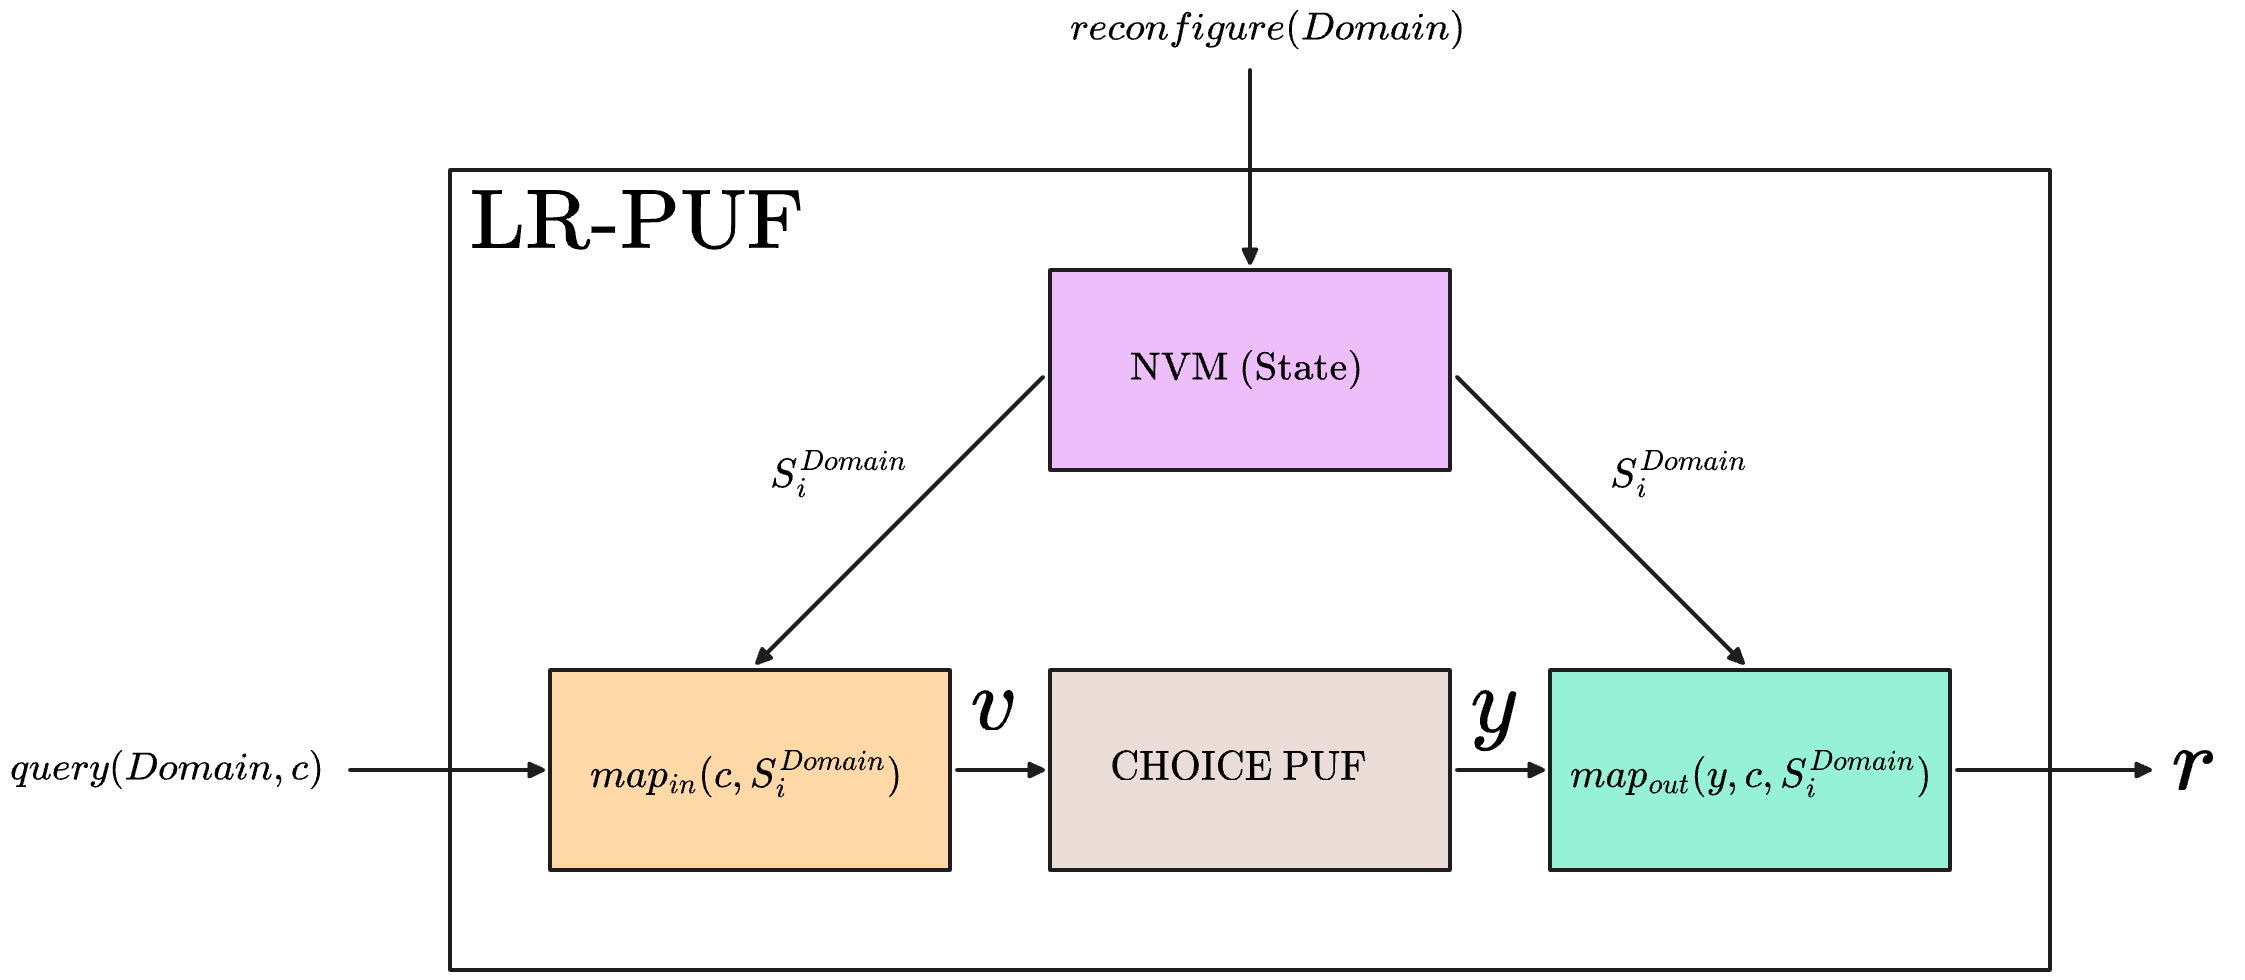
\includegraphics[width=1\linewidth]{img/LR-PUF-Diagram.png}
    \caption{LR-PUF Diagram}
    \label{fig:LR-PUF-Diagram}
\end{figure}

Our chosen LR-PUF architecture can be found in figure \ref{fig:LR-PUF-Diagram}. The LR-PUF augments the CHOICE PUF by using a state that is applied on the incoming challenges through the $map_{in}$ function and on the outgoing responses through the $map_{out}$ function. Calling the $reconfigure$ function changes the state and by extension the CRP behavior of the LR-PUF. Before explaining each of these functions, we need to first clarify the variables shown in the diagram as follows:
\begin{itemize}
    \item $Domain$: We keep a state for each domain or server that the user is connected to. We use the terms server and domain interchangeably.
    \item $S_i^{Domain}$: The current state $i$ associated with some domain. In practice, this state could be any random sequence of bits or integer. It is stored in non-volatile memory, and as per the LR-PUF specification, an attacker with access to this state value cannot use it to uncover the responses of the underlying CHOICE-PUF.
    \item $c$: The outer challenge that is used to query the LR-PUF. As we will see later in the protocol phases, this challenge is to be generated by the server. In practice, it can be any random integer.
    \item $v$: The inner challenge to which the outer challenge $c$ is mapped by calling $v = map_{in}(c, S_i^{Domain})$. This inner challenge is one of the valid challenges uncovered after running the one-time initialization outlined in algorithm \ref{alg:CPUF-one-time-init}. 
    \item $y$: The raw response of the CHOICE-PUF after querying it with challenge $v$.
    \item $r$: The final response of the LR-PUF that will be used as a seed for key generation. It is the result of using the state and $y$ through $r = map_{out}(y, c, S_i^{Domain})$, $c$ is used here to avoid getting the same response twice for the different outer challenges $c_i$ and $c_j$ that would map to the same inner challenge $v$ and give the same response $y$ under some state, because the CHOICE PUF has a limited number of possible challenges and outputs we want to avoid this edge case where two challenges would produce the same response by adding $c$ as input to the $map_{out}$ function.
\end{itemize}

\subsubsection{The $map_{in}$ function}
The input mapping function $map_{in}(c, S_i^{Domain})$ (Algorithm \ref{alg:LRPUF-mapin}) is responsible for translating an arbitrary external challenge $c$ into a valid CHOICE PUF challenge $v \in \mathcal{V}$. It defines a mapping from the set of positive integers $\mathbb{Z}^{+}$ into the set of valid challenges $\mathcal{V}$. The function first derives an index $idx$ by hashing the current domain state with the external challenge and calculating the remainder over the total number of valid challenges to get an index within that range. Then this index is used to select the valid challenge from the set $\mathcal{V}$. This ensures that only valid challenges are used to query the CHOICE PUF and hides the complexity of the CHOICE PUF from the server by allowing it to use any arbitrary challenge $c$. As we will see in a later section explaining the protocol, this challenge $c$ would act similar to a session identifier.

\begin{algorithm}[ht!]
\caption{$map_{in}(c, S_i^{Domain})$}
\begin{algorithmic}[1]
    \Require Challenge $c$, domain state $S_i^{Domain}$, valid challenges set $\mathcal{V}$ stored in NVM
    \Ensure  Mapped challenge $v \in \mathcal{V}$
    \State $idx \leftarrow H(S_i^{Domain} \mathbin\| c) \bmod |\mathcal{V}|$
    \State $v \leftarrow \mathcal{V}[idx]$
    \State \Return $v$
\end{algorithmic}
\label{alg:LRPUF-mapin}
\end{algorithm}

\subsubsection{The $map_{out}$ function}
The output mapping function $map_{out}(y, c, S_i^{Domain})$ (Algorithm \ref{alg:LRPUF-mapout}) is applied on the raw CHOICE PUF response $y$ to produce the final response $r$. It hashes $y$ along with $c$ and the current state $S_i^{Domain}$. Binding $c$ into the output hash prevents response reuse across different challenges since the input space of the CHOICE PUF is quite small and collisions in the $map_{in}$ could happen if queried under the same state.

\begin{algorithm}[ht!]
\caption{$map_{out}(y, c, S_i^{Domain})$}
\begin{algorithmic}[1]
    \Require PUF response $y$, challenge $c$, domain state $S_i^{Domain}$
    \Ensure  Final response $r$
    \State $r \leftarrow H(S_i^{Domain} \mathbin\| c \mathbin\| y)$
    \State \Return $r$
\end{algorithmic}
\label{alg:LRPUF-mapout}
\end{algorithm}

\subsubsection{The $reconfigure$ function}
The reconfiguration function (Algorithm \ref{alg:LRPUF-reconfig}) is the mechanism through which logical reconfigurability is achieved. When called, it generates a random seed using a true random number generator (TRNG) and records the current timestamp. Then it distinguishes between two cases. If no state exists for the given domain, an initial state $S_0^{Domain}$ is derived by selecting a challenge $v$ from  $\mathcal{V}$ using the random seed, then the CHOICE PUF is queried with this challenge $v$ to obtain a response $y$, after which we hash $v$, $y$, the seed and the current timestamp to produce $S_0^{Domain}$. If a state already exists for the given domain, a new state $S_{i+1}^{Domain}$ is derived by hashing the current state $S_i^{Domain}$ with the random seed and timestamp, forming a hash chain that evolves the current state. In both cases, the produced state is finally persisted into the NVM to be used in subsequent LR-PUF querying operations.

\begin{algorithm}[ht!]
\caption{$reconfigure(Domain)$}
\begin{algorithmic}[1]
    \Require Domain identifier $Domain$, valid challenges set $\mathcal{V}$ stored in NVM
    \Ensure  NVM updated with new domain state $S_{i+1}^{Domain}$

    \State $S_i^{Domain} \leftarrow NVM.read(Domain)$
    \State $seed \leftarrow TRNG()$
    \State $now \leftarrow readtime()$

    \If{$S_i^{Domain} = null$} \Comment{Initialize the first state for a new domain}
        \State $idx \leftarrow seed \bmod |\mathcal{V}|$
        \State $v \leftarrow \mathcal{V}[idx]$
        \State $y \leftarrow CHOICE\_PUF(v)$
        \State $S_0^{Domain} \leftarrow H(v \mathbin\| y \mathbin\| seed \mathbin\| now)$
        \State $NVM.write(Domain,S_0^{Domain})$
    \Else
        \State $S_{i+1}^{Domain} \leftarrow H(S_{i}^{Domain} \mathbin\| seed \mathbin\| now)$ 
        \State $NVM.write(Domain,S_{i+1}^{Domain})$
    \EndIf
\end{algorithmic}
\label{alg:LRPUF-reconfig}
\end{algorithm}

\subsubsection{The $query$ function}
The query operation (Algorithm \ref{alg:LRPUF-query}) takes a challenge $c$ and a domain identifier $Domain$. It first retrieves the current domain state $S_i^{Domain}$ associated with the given domain from NVM. Then $c$ is passed along with $S_i^{Domain}$ to $map_{in}$ to get a valid challenge $v$. After that, $v$ is used to query the CHOICE PUF and get a response $y$. Finally $y$ is passed to the $map_{out}$ function along with $c$ and $S_i^{Domain}$ to produce the final response $r$.

\begin{algorithm}[ht!]
\caption{$query(c,Domain)$}
\begin{algorithmic}[1]
    \Require Domain identifier $Domain$, challenge $c$
    \Ensure  Response $r$ 
    \State $S_i^{Domain} \leftarrow NVM.read(Domain)$
    \State $v \leftarrow map_{in}(c, S_i^{Domain})$
    \State $y \leftarrow \textsc{CHOICE\_PUF}(v)$
    \State $r \leftarrow map_{out}(y,c, S_i^{Domain})$
    
    \State \Return $r$
\end{algorithmic}
\label{alg:LRPUF-query}
\end{algorithm}

The binding of both mapping functions to the domain state is what enables logical reconfigurability. By invoking $reconfigure(Domain)$, the state is updated, causing all subsequent queries to the LR-PUF under the same domain to produce entirely different responses without any modifications to the underlying weak CHOICE PUF. 

\subsection{Error Correction Strategy}

Since the outputs of the CHOICE PUF can be noisy, a robust error correction strategy is needed. A fuzzy commitment scheme utilizing a BCH code \cite{BOSE196068} was used.

A BCH code is a cyclic error-correction code parameterized by a codeword length $n$, a message length $k$, and a correction capacity $t$. Given a $k$-bit message $W$, $encode_{BCH}(W)$ appends $(n - k)$ parity bits stored as $ECC$, where $W||ECC$ make up the codeword. During decoding, $decode_{BCH}(W', ECC)$ uses those parity bits to locate and correct up to $t$ bit flips in the noisy word $W'$ and obtain the original $W$.



The error correction strategy for the LR-PUF involves two operations: enrollment and querying. 
\subsubsection{Enrollment}
The enrollment operation is described with the $enroll_{BCH}$ function (Algorithm \ref{alg:PUF-BCH-Enroll}). This is what is actually used to generate a key using the LR-PUF. At first, it takes as input the $Domain$, the outer challenge $c$ and how many times $vote\_count$ to query the CHOICE-PUF to determine a stable response using bit-wise majority voting. Since this enrollment process usually occurs when we want to generate a key for the first time or when we want to rotate keys, the $reconfigure$ function must run to ensure that we have a new state $S_i^{Domain}$. Then this state is used to map the outer challenge $c$ to a valid inner challenge $v$ using the $map_{in}$ function. This challenge $v$ is used to query the CHOICE PUF $vote\_count$ times to determine using bit-wise majority voting the stable PUF response $y$. After this, a secret value $W$ is generated by hashing the state $S_i^{Domain}$, the outer challenge $c$, the PUF response $y$ and the current timestamp. This $W$ value is what will be error-corrected as part of the fuzzy commitment scheme. It was generated this way to make sure that it is sufficiently random. Then $W$ is encoded using BCH error correction to produce the parity bits $ECC$, which are stored in NVM. Helper data $helper = y \oplus W$ is also stored. This is done so that during querying, a noisy PUF response $y'$ can be XORed with $helper$ to recover a noisy version of $W$ which $ECC$ can correct. Finally, $W$ is given to the $map_{out}$ function along with the outer challenge $c$ and the current state $S_i^{Domain}$ to obtain the final response $r$ which can be used as a seed for key generation.

\begin{algorithm}[ht!]
\caption{$enroll_{BCH}(Domain, c, vote\_count)$}
\begin{algorithmic}[1]
    \Require Domain identifier $Domain$, challenge $c$, bit-wise majority voting count $vote\_count$
    \Ensure  Response $r$ (seed) 
    \State $reconfigure(Domain)$
    \State $S_i^{Domain} \leftarrow NVM.read(Domain)$
    \State $v \leftarrow map_{in}(c, S_i^{Domain})$
    \State \(\triangleright\) Bit-wise majority voting to determine the CHOICE PUF response $y$
 \State $\text{ones}[0..63] \leftarrow \mathbf{0}$
  \For{$i = 1$ \textbf{to} $vote\_count$}
      \State $m \leftarrow \textsc{CHOICE\_PUF}(v)$
      \For{$b = 0$ \textbf{to} $63$}
          \State $\text{ones}[b] \leftarrow \text{ones}[b] + m[b]$
      \EndFor
  \EndFor
 \For{$b = 0$ \textbf{to} $63$}
      \If{$\text{ones}[b] \cdot 2 \geq vote\_count$}
          \State $y[b] \leftarrow 1$
      \Else
          \State $y[b] \leftarrow 0$
      \EndIf
  \EndFor
    \State \(\triangleright\) Fuzzy commitment
    \State $W \leftarrow H(S_i^{Domain}||c||y||now)$
    \State $ECC \leftarrow encode_{BCH}(W)$
    \State $helper \leftarrow y \oplus W$
    \State $NVM.write(Domain, ECC)$
    \State $NVM.write(Domain, helper)$
    \State $r \leftarrow map_{out}(W,c, S_i^{Domain})$ 
    \State \Return $r$
\end{algorithmic}
\label{alg:PUF-BCH-Enroll}
\end{algorithm}



\subsubsection{Querying}
The query operation is described with the $query_{BCH}$ function  (Algorithm \ref{alg:PUF-BCH-Query}). It takes as input the domain identifier $Domain$ and the outer challenge $c$. To recover the response $r$ generated with $enroll_{BCH}$, we first fetch $S_i^{Domain}$, $helper$ and $ECC$ from NVM using $Domain$. Then, $map_{in}$ is used to get the valid challenge $v$ using $c$ and $S_i^{Domain}$. This valid challenge $v$ is used to query the CHOICE PUF once to get a response $y'$. Unlike enrollment, no majority voting is performed here, so $y'$ may be noisy. $W'$ is obtained by taking $y' \oplus helper$, and $decode_{BCH}(W', ECC)$ corrects the errors to recover the original $W$, given that the noise is within the error-correction capacity of the BCH code. Finally, $W$ is given to $map_{out}$ along with $c$ and $S_i^{Domain}$ to obtain the original $r$ so that we can use it as a seed to recover the previously enrolled key.



\begin{algorithm}[ht!]
\caption{$query_{BCH}(Domain, c)$}
\begin{algorithmic}[1]
    \Require Domain identifier $Domain$, challenge $c$.
    \Ensure  Response $r$ (seed) 
    \State $S_i^{Domain},helper,ECC \leftarrow NVM.read(Domain)$
    \State $v \leftarrow map_{in}(c, S_i^{Domain})$
    \State $y' \leftarrow CHOICE\_PUF(v)$
    \State $W' \leftarrow y' \oplus helper $
    \State $W \leftarrow decode_{BCH}(W', ECC)$
    \State $r \leftarrow map_{out}(W,c, S_i^{Domain})$ 
    \State \Return $r$
\end{algorithmic}
\label{alg:PUF-BCH-Query}
\end{algorithm}

\subsection{Justifications for using a PUF}
Since the question of "Why use a PUF specifically and not some other conventional secure storage primitive?" is one that will be asked when looking at the dongle design, an answer is in order. The design choice to use a PUF rather than some other secure storage primitive, like a TPM or encrypted flash memory, is a deliberate one. Although these other mechanisms are mature, standardized and widely deployed, they all share one common property: the secret physically resides somewhere on the die at all times. The PUF approach does not have this property. This allows it to provide several benefits that align with REPUSH's threat model and design goals.

First, there is no key at rest. The private key is generated on demand and discarded immediately after use. An attacker that obtains a powered-off dongle finds no secret to extract. Although physical attacks are out of scope for our threat model, this property could be useful in future iterations of the REPUSH protocol that would consider physical attacks as well.

Second, there is no key provisioning step needed to be taken by the manufacturer. Other schemes, where a key is stored, introduce a trust dependency on the supply chain of the dongle. With a PUF, the cryptographic identity emerges from the chip fabric itself without requiring explicit introduction of the secret by some manufacturer.

The second benefit is more in line with REPUSH's security goals as we are trying to reduce the dependency on third parties and also makes more sense economically since no provisioning step is needed for manufacturing the dongles.

\section{Protocol Design}
The REPUSH protocol is composed of three phases.
The following notations are used: $\{m\}_K$ denotes encryption of $m$ with key $K$, $[m]_K$ denotes a signature on $m$ with key $K$,
and $||$ is concatenation. The steps shown as $\boldsymbol{\langle x \rangle}$ may fail, in which case the red arrow branch is taken.
The diagrams contain a high-level overview of the process, each function is described in more detail in its respective algorithm figure. In the algorithms pseudo-code, querying the LR-PUF is indicated with $query_{BCH}(Challenge, Domain)$ (Algorithm \ref{alg:PUF-BCH-Query}).

\subsection{Phase 1: Enrollment and Login}
The first phase of REPUSH initiates a session between the dongle and the server. This phase has two objectives:
\begin{enumerate}
    \item Mutual authentication by authenticating the server to the dongle and user using a CA certificate, and then authenticating the user and the dongle to the server with a username and password. 
    \item Establishing a dongle-bound asymmetric key pair $SK_0$ and $PK_0$ to be used for the first session.
\end{enumerate}

\begin{figure}
    \centering
    \includegraphics[width=1.25\linewidth]{img/REPUSH-1.png}
    \caption{Phase 1: Enrollment and Login}
    \label{fig:REPUSH-phase-1}
\end{figure}

The first phase described in figure \ref{fig:REPUSH-phase-1} is composed of the following steps:
\paragraph{$\boldsymbol{(1)}$} The user initiates a dongle login request with the server using the browser. As opposed to a normal login request, the dongle login request tells the browser that the user wants to associate a dongle with the session.

\paragraph{$\boldsymbol{(2)}$} Consequently, the server runs the function $DongleLogin()$ (Algorithm \ref{alg:dongle-login}) to fetch the $Cert$ and generate a $LoginPayload$. The $Cert$ associates the server's $Domain$ with its public key $PK_{Server}$ using a signature signed by the CA, the dongle will later use this $Cert$ to authenticate the server. The $LoginPayload$ is also intended for the dongle, it contains the following:
\begin{itemize}
    \item The string \verb|"login"| that will tell the dongle to perform a login operation.
    \item A randomly generated challenge for the LR-PUF $C_\text{Session}^0$ that will be used by the dongle to generate the asymmetric key pair $(SK_0,PK_0)$ for the first session.
    \item A nonce $N$ to avoid playback attacks and to track the requests.
    \item A login payload composed of a signature on $\verb|"login"|||C_\text{Session}^0||N$ with $SK_\text{Server}$ to prove to the dongle that this payload is indeed coming from the expected domain or server.
\end{itemize}
\begin{algorithm}[ht!]
\caption{$DongleLogin()$}
\begin{algorithmic}[1]
    \Require Incoming dongle login request
    \Ensure  $(\mathit{Cert}, \mathit{LoginPayload})$ returned to the browser.

    \State $C^0_{\text{Session}} \leftarrow TRNG()$
    \State $N \leftarrow TRNG()$
    \State $Cert \leftarrow (Domain||PK_\text{Server},[Domain||PK_\text{Server}]_{SK_{CA}})$
    \State $\mathit{LoginPayload} \leftarrow
            (\texttt{"login"} || C^0_{\text{Session}} || N,
            [\texttt{"login"} || C^0_{\text{Session}} || N]_{\mathit{SK}_{\text{Server}}})$
    \State \textbf{return} $(\mathit{Cert}, \mathit{LoginPayload})$
\end{algorithmic}
\label{alg:dongle-login}
\end{algorithm}
\paragraph{$\boldsymbol{(3)}$} The server sends back $Cert$ and $LoginPayload$ to the browser, then the browser forwards them to DOMAN (via HTTP).
\paragraph{$\boldsymbol{(4)}$} DOMAN sends an "Enroll" request to the dongle (via a Serial interface) for the dongle to run the $DongleEnroll(Cert, LoginPayload)$ function (Algorithm \ref{alg:dongle-enroll}).

\begin{algorithm}[ht!]
\caption{$DongleEnroll(Cert, LoginPayload)$}
\begin{algorithmic}[1]
    \Require Enroll command with $(\mathit{Cert}, \mathit{LoginPayload})$ received from the DOMAN.
    \Ensure  $(\mathit{LoginToken}, Domain, \mathit{SignedPayload})$ returned to the browser,
             or an error.

    \State $V_{\text{Server}} \leftarrow Verify(Cert, PK_{CA})$
    \If{$V_{\text{Server}} = \text{failed}$}
        \State \textbf{return} "Certificate verification failed"
    \EndIf
    \State $Domain, PK_{\text{Server}} \leftarrow Cert$
    \State $V_{\text{Payload}} \leftarrow Verify(LoginPayload, PK_{\text{Server}})$
    \If{$V_{\text{Payload}} = \text{failed}$}
        \State \textbf{return} "Payload verification failed"
    \EndIf
    \State $P, Username, Password \leftarrow UserLogin(Domain)$
    \If{$P = \text{reject}$}
        \State \textbf{return} "User rejected login request"
    \EndIf
%    \State $reconfigure(Domain)$ \Comment{Initializes $S_0^{Domain}$}
    \State $C^0_{\text{Session}} \leftarrow LoginPayload$
    \State $seed_0 \leftarrow enroll_{BCH}(Domain, C^0_{\text{Session}}, 10)$
    \State $SK_0, PK_0 \leftarrow KeyGen(seed_0)$
    \State $LoginToken \leftarrow \{Username||Password||PK_0\}_{PK_{\text{Server}}}$
    \State $SignedLoginPayload \leftarrow [LoginPayload]_{SK_0}$
    \State \textbf{return} $(LoginToken, Domain, SignedLoginPayload)$
\end{algorithmic}
\label{alg:dongle-enroll}
\end{algorithm}
\paragraph{$\boldsymbol{\langle 5\rangle}$} The dongle first verifies if the provided $Cert$ was actually signed by the $CA$, if this step fails, the login request is rejected by the dongle.
\paragraph{$\boldsymbol{\langle 6\rangle}$} The dongle extracts $PK_\text{Server}$ from $Cert$ and uses it to verify if the signed $LoginPayload$ is indeed coming from the server. If this step fails, the login request is rejected by the dongle.
\paragraph{$\boldsymbol{\langle 7\rangle}$} The $Domain$ extracted from $Cert$ is displayed on the dongle's touch screen (Figure \ref{fig:login-screens}), where the user is expected to read it and verify if it is the intended domain where they wish to login. The user has two options, either to accept or reject this login request. This here concludes the part where the dongle authenticates the server. The displayed $Domain$ was extracted from $Cert$ and is guaranteed to actually be associated with $PK_\text{Server}$ because of the CA's signature on it. Furthermore, if a compromised host tries fooling the dongle with some other $Domain$ here, the user will catch on because the $Domain$ is displayed on the screen and requires approval. 
\paragraph{$\boldsymbol{\langle 8\rangle}$} The user is prompted to enter their $Username$ and $Password$ for the $Domain$ on the dongle's touch screen (Figure \ref{fig:login-screens}). Alternatively, the dongle could be used as a password manager in this step to make it more practical for the user so that they do not have to manually enter their credentials every time, but this use-case is currently out of scope for REPUSH's focus on protecting against session hijacking. The user can still cancel at this point, in which case the login request is rejected by the dongle.
\begin{figure}
    \centering
    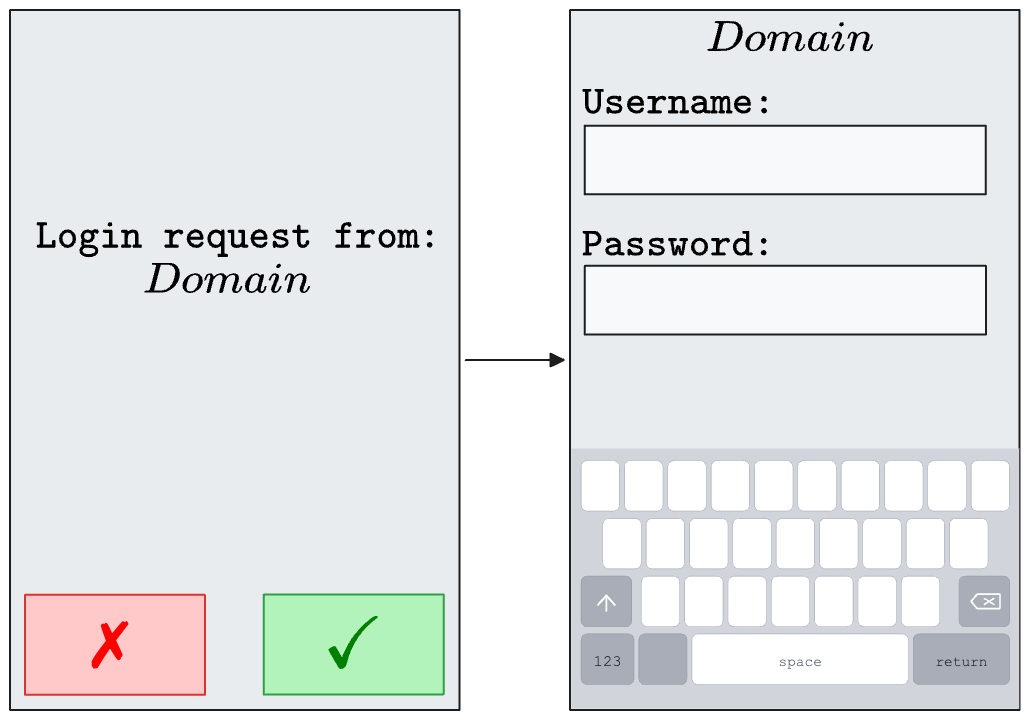
\includegraphics[width=0.5\linewidth]{img/touch-screen-login.png}
    \caption{User prompts for login on the dongle's touch screen}
    \label{fig:login-screens}
\end{figure}
\paragraph{$\boldsymbol{(9)}$} The LR-PUF is queried using $C_\text{Session}^0$ to generate the key pair $(SK_0, PK_0)$, this is done by first running $enroll_{BCH}(Domain, C_\text{Session}^0,10)$ (Algorithm \ref{alg:PUF-BCH-Enroll}) which will in turn initialize $S_0^{Domain}$ and perform the necessary error-encoding to get as a response $seed_0$, this seed is then given to some key generation algorithm to get an asymmetric key pair $(SK_0, PK_0)$.
\paragraph{$\boldsymbol{(10)}$} The user-provided $Username$ and $Password$ along with the generated public key $PK_0$ are encrypted using the server public key $PK_\text{Server}$ to create $LoginToken$. This $LoginToken$ is encrypted with $PK_\text{Server}$ to ensure that only the server can decrypt it and access the user's password within.
\paragraph{$\boldsymbol{(11)}$} The provided $LoginPayload$ is signed with $SK_0$ to further confirm to the server that the dongle did in fact receive the $LoginPayload$ and the $PK_0$ can be used for the first session.
\paragraph{$\boldsymbol{(12)}$} $LoginToken$, $Domain$ and $[LoginPayload]_{SK_0}$ are returned to DOMAN, then DOMAN sends them to the browser, and finally the browser sends $LoginToken$ and $[LoginPayload]_{SK_0}$ to the server. The server then runs the function $VerifyLogin(LoginToken, [LoginPayload]_{SK_0})$ (Algorithm \ref{alg:verify-login}).

\begin{algorithm}[ht!]
\caption{$VerifyLogin(LoginToken, [LoginPayload]_{SK_0})$}
\begin{algorithmic}[1]
    \Require $LoginToken$ and $[LoginPayload]_{SK_0}$.
    \Ensure  $LoginAck$ and session $Cookies_0$ returned to the browser,
             or an error.

    \State $D_{LoginToken} \leftarrow Decrypt(LoginToken, SK_{\text{Server}})$
    \If{$D_{LoginToken} = \text{failed}$}
        \State \textbf{return} "Reject login request"
    \EndIf
    \State $Username, Password, PK_0 \leftarrow D_{LoginToken}$
    \State $auth \leftarrow Authenticate(Username, Password)$ \Comment{optional: extra MFA}
    \If{$auth = \text{failed}$}
        \State \textbf{return} "Reject login request"
    \EndIf
    \State $V_{Payload} \leftarrow Verify(SignedPayload, PK_0)$
    \If{$V_{Payload} = \text{failed}$}
        \State \textbf{return} "Reject login request"
    \EndIf
    \State $LoginAck \leftarrow [PK_0||C_{Session}^0||Domain]_{SK_{\text{Server}}}$
    \State $store(PK_0,\ C^0_{\text{Session}})$
    \State $Cookies_0 \leftarrow GenerateCookies()$
    \State $t^{Session}_{\text{last}} \leftarrow Now()$ 
    \State $t^{Session}_{\text{start}} \leftarrow Now()$
    \State \textbf{return} $(LoginAck, Cookies_0)$
\end{algorithmic}
\label{alg:verify-login}
\end{algorithm}

\paragraph{$\boldsymbol{\langle 13\rangle}$ and $\boldsymbol{\langle 14\rangle}$} The server decrypts $LoginToken$ using $SK_\text{Server}$ to get $Username$, $Password$ and $PK_0$ from it. If one of these steps fails, the login request is rejected.
\paragraph{$\boldsymbol{\langle15\rangle}$} The server checks the validity of the provided $Username$ and $Password$ against its internal database, optionally, an extra multi-factor authentication step could be added here for extra security. If this step fails, the login request is rejected.
\paragraph{$\boldsymbol{\langle16\rangle}$} $[LoginPayload]_{SK_0}$ is verified using $PK_0$ for the server to verify that $LoginPayload$ was indeed received and signed by the dongle and that $PK_0$ has been agreed as the first key for this session. If this step fails, the login request is rejected.
\paragraph{$\boldsymbol{(17)}$} A login acknowledgment $LoginAck$ is created by signing $PK_0||C_{Session}^0||Domain$ with $SK_\text{Server}$. This login acknowledgment will later be sent to the dongle to acknowledge the login.
\paragraph{$\boldsymbol{(18)}$} A session is created by associating $PK_0$ with $C_{Session}^0$ and generating $Cookies$. 
\paragraph{$\boldsymbol{(19)}$} $Cookies$ and $LoginAck$ are sent to the browser.
\paragraph{$\boldsymbol{(20)}$} $Cookies$ stay in the browser, and $LoginAck$ and $Domain$ are sent to the dongle for it to run $AckEnroll(Domain, LoginAck)$ (Algorithm \ref{alg:ack-enroll}).
\begin{algorithm}[ht!]
\caption{$AckEnroll(Domain, LoginAck)$}
\begin{algorithmic}[1]
    \Require $(Domain, LoginAck)$ received from the browser.
    \Ensure  Login success on valid acknowledgment returned to the browser and persisted state
             $(Domain, S_0^{Domain}, C^0_{\text{Session}}, PK_0)$ in the dongle. Otherwise, a login error is returned to the browser.
     \State $V_{LoginAck} \leftarrow Verify(LoginAck, PK_0||C^0_{\text{Session}}||Domain, PK_{\text{Server}})$
    \If{$V_{LoginAck} = \text{failed}$}
        \State \textbf{return} "Login not acknowledged"
    \EndIf
    \State $store(Domain, S_0^{Domain}, C^0_{\text{Session}}, PK_0)$
    \State \textbf{return} "Login success"
\end{algorithmic}
\label{alg:ack-enroll}
\end{algorithm}
\paragraph{$\boldsymbol{\langle21\rangle}$} The signature $LoginAck$ is verified using $PK_{Server}$ and the already established $PK_0$, $C_{Session}^0$ and $Domain$. If this step fails a login error is returned to the browser.
\paragraph{$\boldsymbol{(22)}$} The tuple $(Domain, S_0^{Domain}, C^0_{\text{Session}}, PK_0)$ is stored on the dongle for it to be used in the next phase of the protocol.

\paragraph{$\boldsymbol{(23)}$} On login success returned from the dongle, the tuple $(Domain, Cookies)$ is stored on the browser.

By the end of this first phase, we would have securely established $PK_{Server}$ on the dongle thanks to the CA certificate, and $PK_0$ on the server-side with the $LoginToken$ which associates $Username$ and $Password$ with $PK_0$. The dongle used $Cert$ as trust anchor, whilst the server used the user's credentials as a trust anchor for accepting $PK_0$. We will now see in the next phase of the protocol how $PK_0$ or any subsequent $PK_i$ can be used for continuous session validation.

\subsection{Phase 2: Operation Phase}
The operation phase has two concurrent modes of operation, the first is similar to PUSH's approach to continuous session validation, where requests are allowed as long as the cookies are provided for a certain validity window, after which the dongle is requested to sign a nonce with $SK_i$ given $C_{Session}^i$ to prove ownership of the dongle. REPUSH adopts this approach for non-sensitive requests. For sensitive requests, the second mode of operation is in order. In which the request must be approved by the user on the dongle's screen and then signed with $SK_i$. 
\subsubsection{Non-sensitive Requests Operation}
What counts as "non-sensitive" is a judgment to be made by the server or application. For example, read-only navigation, pagination, search queries and fetching static content can be considered as "non-sensitive". 

\begin{figure}
    \centering
    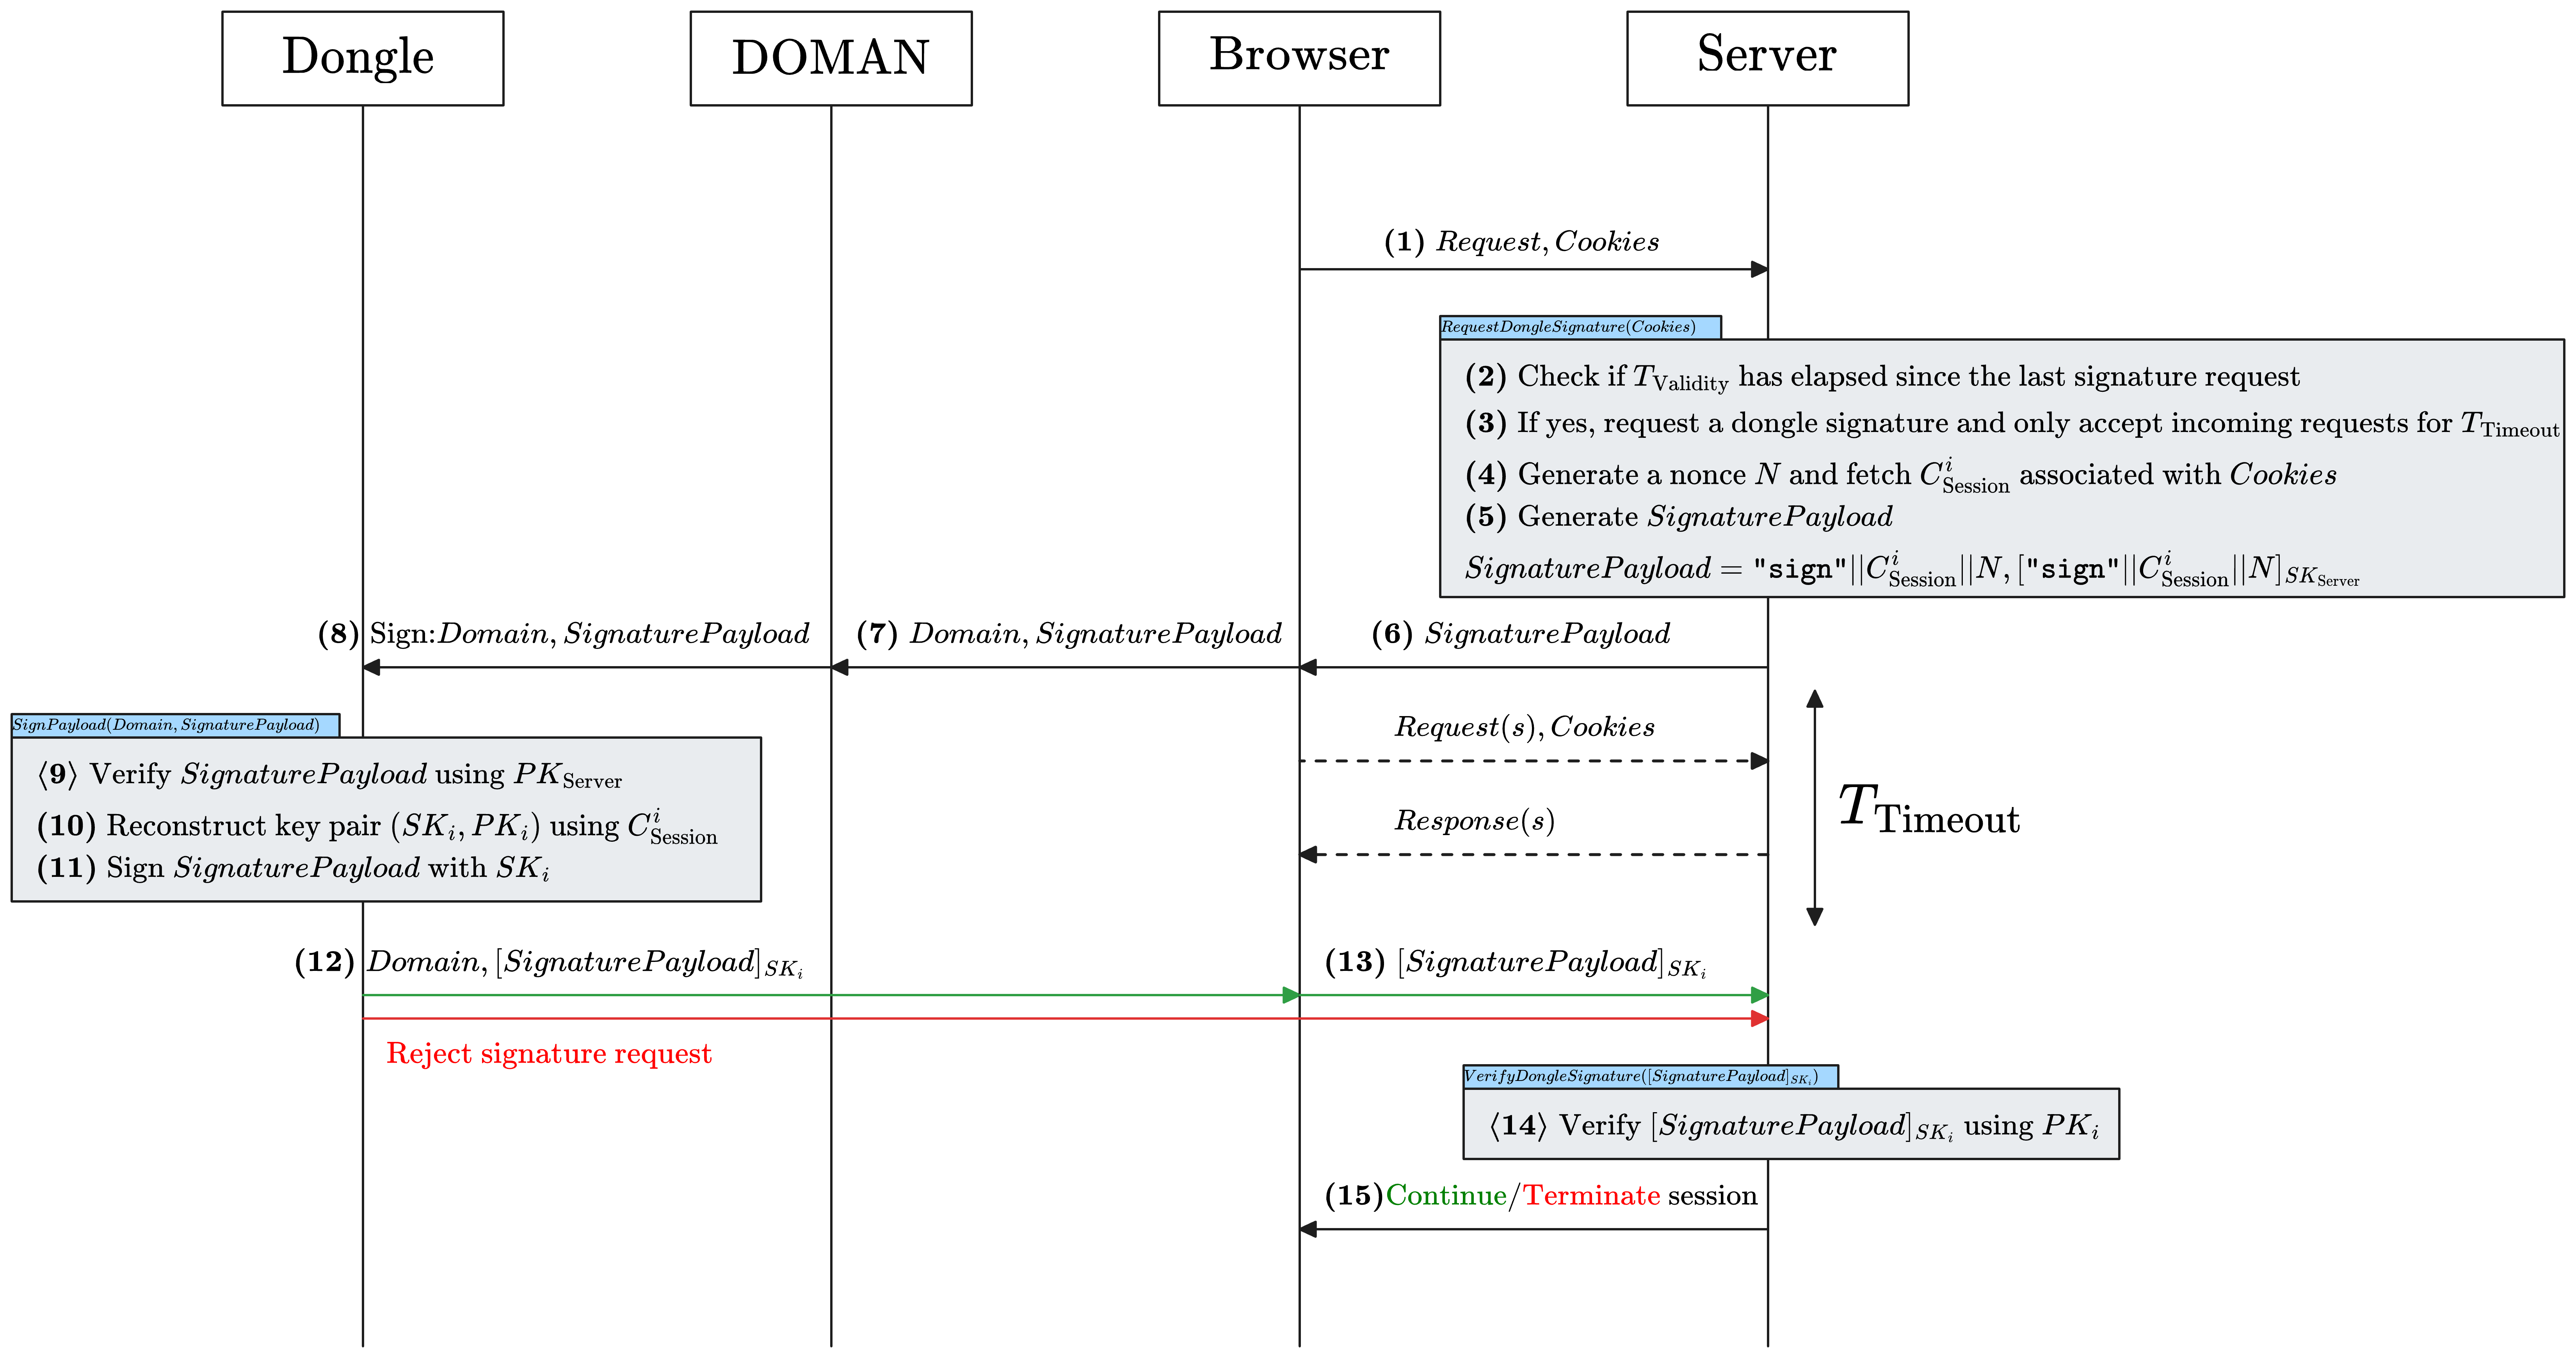
\includegraphics[width=1.25\linewidth]{img/REPUSH-2-Non-Sensitive.png}
    \caption{Phase 2: Operation Phase - Non-sensitive Requests}
    \label{fig:REPUSH-phase-2-non-sensitive}
\end{figure}

The continuous session validation for non-sensitive requests is defined in Figure \ref{fig:REPUSH-phase-2-non-sensitive}. Here the following time variables are used to determine session validity and when to request proof of dongle ownership:
\begin{itemize}
    \item $T_\text{Validity}$: The maximum time interval within which the server accepts incoming requests without a fresh dongle signature. The smaller this interval, the sooner a hijacked session is caught, but at the cost of more latency.
    \item $T_\text{Timeout}$: The grace time window within which the server accepts incoming requests after requesting a fresh dongle signature. If no valid signature arrives by the end of this time window, the session is terminated.
    \item $t^{Session}_{\text{last}}$: The timestamp of the last successful dongle validation for the current session, it is initialized as $Now()$ when Phase 1 completes. 
    \item $t^{Session}_\text{deadline}$: The timestamp deadline by which the currently requested dongle signature must arrive, it is set to $Now() + T_\text{Timeout}$ when a dongle signature is requested. 
\end{itemize}

This phase is composed of the following steps: 

\paragraph{$\boldsymbol{(1)}$} The browser makes some request to the server and presents the $Cookies$ along. On every request received, the server will run the function $RequestDongleSignature(Cookies)$ (Algorithm \ref{alg:request-dongle-signature}). 
\begin{algorithm}[ht!]
\caption{$RequestDongleSignature(Cookies)$}
\begin{algorithmic}[1]
    \Require Incoming request with $Cookies$, and
             per-session state including $t^{Session}_{\text{last}}$ and $C^i_{\text{Session}}$.
    \Ensure  $SignaturePayload$ returned to the browser when revalidation is due;
             otherwise the request is served normally.
    \State $\Delta_\text{Elapsed} \leftarrow Now() - t^{Session}_{\text{last}}$
    \If{$\Delta_\text{Elapsed} < T_{\text{Validity}}$}
        \State \textbf{return} \texttt{NULL} \Comment{still within the validity window}
    \EndIf
    \State $t^{Session}_{\text{deadline}} \leftarrow Now() + T_{\text{Timeout}}$
    \State $N \leftarrow TRNG()$
    \State $C^i_{\text{Session}} \leftarrow Fetch(Cookies)$
    \State $SignaturePayload \leftarrow
            (\texttt{"sign"} || C^i_{\text{Session}} || N,
            [\texttt{"sign"} || C^i_{\text{Session}} || N]_{SK_{\text{Server}}})$
    \State $TriggerTerminateOn(t_\text{deadline}^{Session})$
    \State \textbf{return} $SignaturePayload$
\end{algorithmic}
\label{alg:request-dongle-signature}
\end{algorithm}
\paragraph{$\boldsymbol{(2)}$ and $\boldsymbol{(3)}$} Before processing the request, the server checks if $T_\text{Validity}$ has elapsed since the last signature by checking if $Now() - t_\text{last}^{Session} < T_\text{Validity}$. If this condition is true, then no verification is needed for now and the request is processed. Otherwise, $t_\text{deadline}^{Session}$ is set to $Now() + T_\text{Timeout}$, a signature is requested from the dongle and requests continue to be served up to $t_\text{deadline}^{Session}$.
\paragraph{$\boldsymbol{(4)}$ and $\boldsymbol{(5)}$} To request a signature from the dongle, a nonce $N$ is generated and the challenge $C_\text{Session}^i$ associated with the cookies is fetched to generate $SignaturePayload = (\texttt{"sign"} || C^i_{\text{Session}} || N,
            [\texttt{"sign"} || C^i_{\text{Session}} || N]_{SK_{\text{Server}}})$. Then a trigger on the server is started which will terminate the session when the timestamp reaches $t_\text{deadline}^{Session}$.
\paragraph{$\boldsymbol{(6)}$, $\boldsymbol{(7)}$ and $\boldsymbol{(8)}$} $SignaturePayload$ is sent to the browser. Then the browser sends $Domain$ and $SignaturePayload$ to DOMAN, which then forwards it to the dongle as a signature request to run the function $SignPayload(Domain, SignaturePayload)$ (Algorithm \ref{alg:sign-payload}) 
\begin{algorithm}[ht!]
\caption{$SignPayload(Domain, SignaturePayload)$}
\begin{algorithmic}[1]
    \Require $(Domain, SignaturePayload)$ received from DOMAN.
    \Ensure  $(Domain, [SignaturePayload]_{SK_i})$ returned to the browser, or an error.
    \State $V_{Payload} \leftarrow Verify(SignaturePayload, PK_{\text{Server}})$
    \If{$V_{Payload} = \text{failed}$}
        \State \textbf{return} ``Reject signature request''
    \EndIf
    \State $\texttt{"sign"},\ C^i_{\text{Session}},\ N \leftarrow SignaturePayload$
%    \State $seed'_i \leftarrow LR\text{-}PUF(S_i^{Domain},\ C^i_{\text{Session}})$
%    \State $seed_i \leftarrow ErrorCorrect(seed'_i)$
    \State $seed_i \leftarrow query_{BCH}(Domain, C^i_\text{Session})$ 
    \State $SK_i,\ PK_i \leftarrow KeyGen(seed_i)$
    \State $[SignaturePayload]_{SK_i} \leftarrow Sign(SignaturePayload, SK_i)$
    \State \textbf{return} $(Domain, [SignaturePayload]_{SK_i})$
\end{algorithmic}
\label{alg:sign-payload}
\end{algorithm}

\paragraph{$\boldsymbol{\langle9\rangle}$} Verify the received $SignaturePayload$ using $PK_\text{Server}$ to make sure that the signature request is coming from the server.

\paragraph{$\boldsymbol{(10)}$} Query the LR-PUF with the $query_{BCH}$ (Algorithm \ref{alg:PUF-BCH-Query}) using the challenge $C_\text{Session}^i$ found within $SignaturePayload$ and $Domain$ to get as a response $seed_i$. Here $seed_i$ was actually error-corrected, so it is identical to the one enrolled in the first phase. Then $KeyGen(seed_i)$ is used to generate the key pair $(SK_i, PK_i)$.

\paragraph{$\boldsymbol{(11)}$} Sign $SignaturePayload$ with $SK_i$ to prove to the server that the dongle possesses the private key $SK_i$ associated with the currently enrolled session public key $PK_i$.

\paragraph{$\boldsymbol{(12)}$ and $\boldsymbol{(13)}$} $Domain$ and $[SignaturePayload]_{SK_i}$ is sent to the browser. Then the browser sends $[SignaturePayload]_{SK_i}$ as a response to the server to prove ownership of the dongle. When received, the server will run the function $VerifyDongleSignature([SignaturePayload]_{SK_i})$ (Algorithm \ref{alg:verify-dongle-signature}).

\begin{algorithm}[ht!]
\caption{$VerifyDongleSignature([SignaturePayload]_{SK_i})$}
\begin{algorithmic}[1]
    \Require Signed payload received from the browser, and
             $PK_i$ and $t^{Session}_{\text{deadline}}$ stored in the session state.
    \Ensure  Session continues on valid and timely signature, otherwise it is terminated.
    \State $V \leftarrow Verify([SignaturePayload]_{SK_i}, SignaturePayload, PK_i)$
    \If{$V = \text{failed}$}
        \State $Terminate(Session)$
        \State \textbf{return} "Terminate session"
    \EndIf
    \State $CancelTerminateOn(t_\text{deadline}^{Session})$
    \State $t^{Session}_{\text{last}} \leftarrow Now()$
    \State \textbf{return} "Continue session"
\end{algorithmic}
\label{alg:verify-dongle-signature}
\end{algorithm}

\paragraph{$\boldsymbol{\langle14\rangle}$} The server verifies $[SignaturePayload]_{SK_i}$ using $PK_i$, and $t^{Session}_\text{last}$ is reset to $Now()$ and the termination trigger on $t_\text{deadline}^{Session}$ is canceled.

\paragraph{$\boldsymbol{(15)}$} The session is terminated if the verification of the received signed payload fails or if the timestamp $t_\text{deadline}^{Session}$ is reached before receiving a valid $[SignaturePayload]_{SK_i}$. Otherwise, the session stays alive. Since $SignaturePayload$ is embedded in the server's response to an active request, every connection presenting the stolen cookies independently receives it and must produce a valid signature on it to keep the session attached to that connection. In other words, a cookie or session can be associated with multiple connections, and each connection must prove ownership of the dongle independently to keep the session attached to it. This is to counter the case where an attacker with stolen cookies would rely on the legitimate verification coming from the user to keep the attacker's session alive. This approach also provides a way to handle normal IP changes caused by the ISP that can happen during a session. 

\subsubsection{Sensitive Request Operation}

\begin{figure}
    \centering
    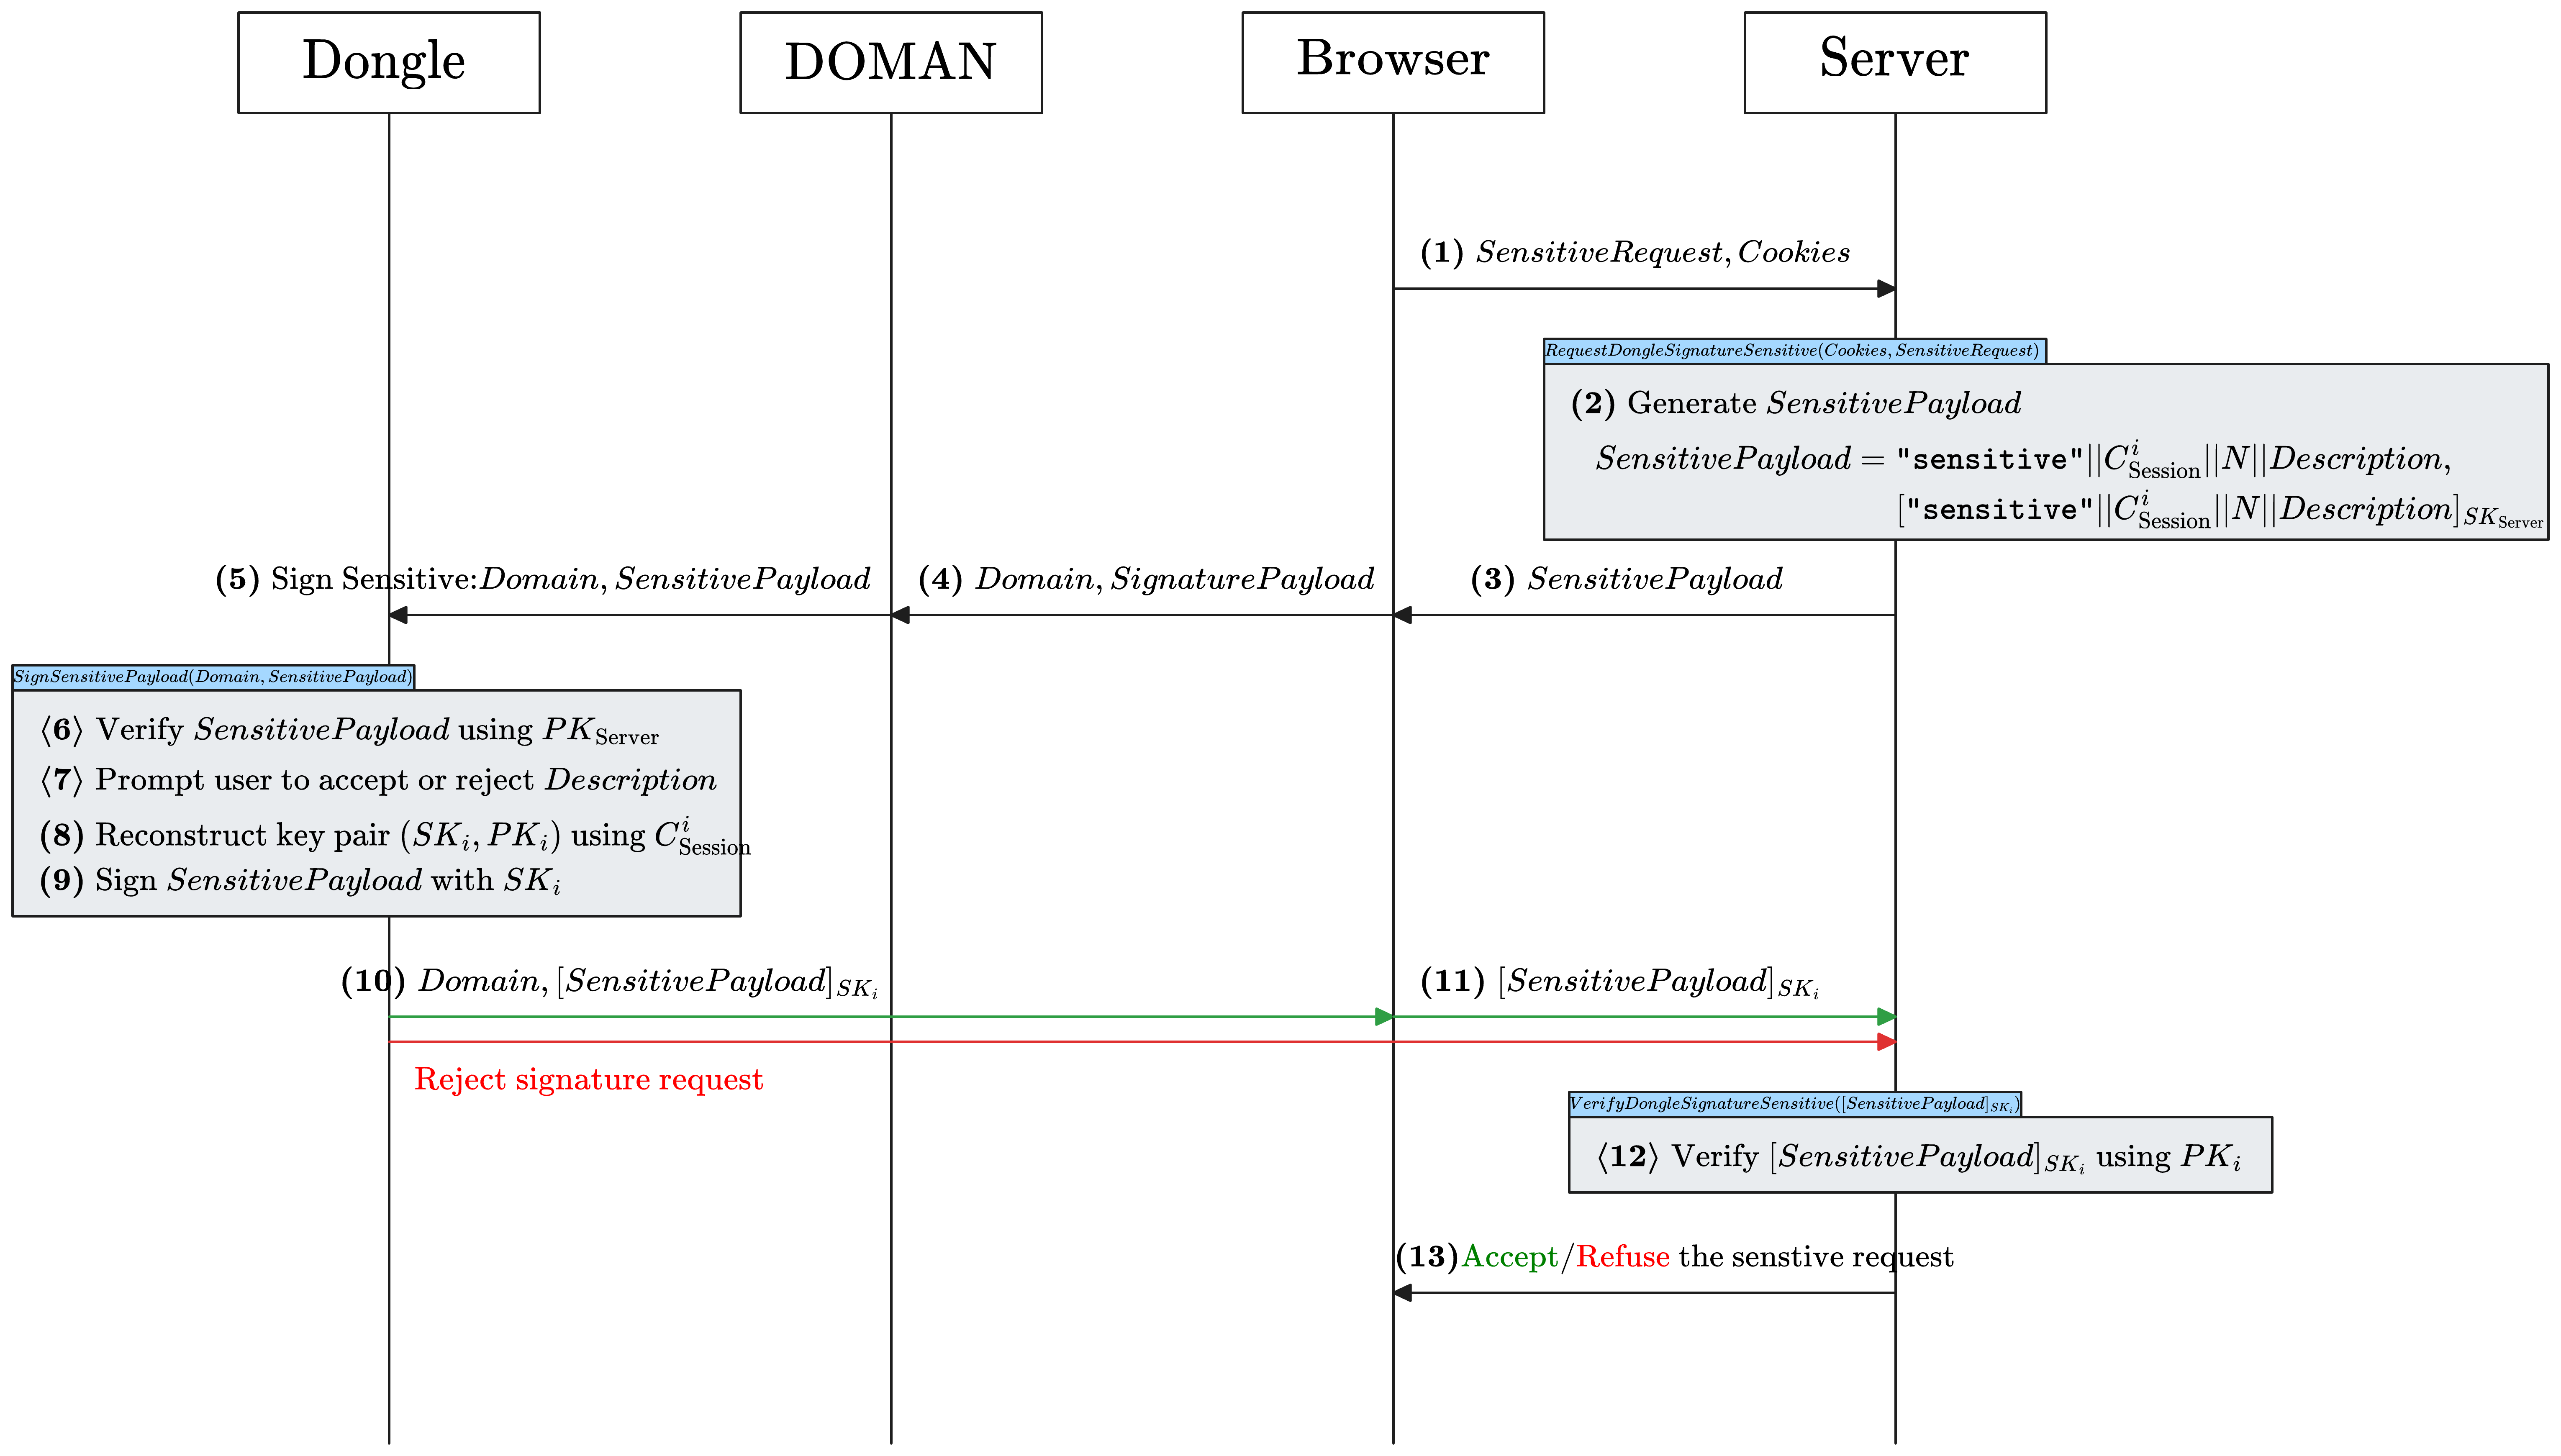
\includegraphics[width=1.25\linewidth]{img/REPUSH-2-Sensitive.png}
    \caption{Phase 2: Operation Phase - Sensitive Requests}
    \label{fig:REPUSH-phase-2-sensitive}
\end{figure}

The second mode of operation occurs in parallel with the previously presented continuous session authentication. It is used to handle sensitive requests. Again, what counts as "sensitive" is a judgment to be made by the server or application. For example, email change, making a post or a comment could be considered as "sensitive". During this phase (Figure \ref{fig:REPUSH-phase-2-sensitive}), the sensitive request must be verified and explicitly accepted by the user on the dongle's screen before it gets signed and sent to the server. This phase is composed of the following steps:

\paragraph{$\boldsymbol{(1)}$} The user through the browser makes some sensitive request to the server and presents the $Cookies$ along. When received, the server runs $RequestDongleSignatureSensitive(Cookies, SensitiveRequest)$ (Algorithm \ref{alg:request-dongle-signature-sensitive}).
\begin{algorithm}[ht!]
\caption{$RequestDongleSignatureSensitive(Cookies, SensitiveRequest)$}
\begin{algorithmic}[1]
    \Require Sensitive application request $SensitiveRequest$ with $Cookies$, and per-session state including $C^i_{\text{Session}}$.
    \Ensure  $SensitivePayload$ returned to the browser.
    \State $N \leftarrow TRNG()$
    \State $C^i_{\text{Session}} \leftarrow Fetch(Cookies)$
    \State $Description \leftarrow Describe(SensitiveRequest)$
    \State $\begin{aligned}[t]
        SensitivePayload \leftarrow (
        &\texttt{"sensitive"} || C^i_{\text{Session}} || N || Description,\\
        &[\texttt{"sensitive"} || C^i_{\text{Session}} || N || Description]_{SK_{\text{Server}}})
        \end{aligned}$
    \State \textbf{return} $SensitivePayload$
\end{algorithmic}
\label{alg:request-dongle-signature-sensitive}
\end{algorithm}
\paragraph{$\boldsymbol{(2)}$} $SensitivePayload$ is generated as: 
$$SensitivePayload= \texttt{"sensitive"} || C^i_{\text{Session}} || N || Description,
        [\texttt{"sensitive"} || C^i_{\text{Session}} || N || Description]_{SK_{\text{Server}}}$$
Where the challenge $C_\text{Session}^i$ is the one associated with the cookies, $N$ is a nonce and $Description$ is derived from the purpose of $SensitiveRequest$.
\paragraph{$\boldsymbol{(3)}$, $\boldsymbol{(4)}$ and $\boldsymbol{(5)}$} $SensitivePayload$ is sent to the browser. Then the browser sends $Domain$ and $SensitivePayload$ to DOMAN, which then forwards it to the dongle as a signature request to run the function $SignSensitivePayload(Domain, SensitivePayload)$ (Algorithm \ref{alg:sign-sensitive-payload}).
\begin{algorithm}[ht!]
\caption{$SignSensitivePayload(Domain, SensitivePayload)$}
\begin{algorithmic}[1]
    \Require $(Domain, SensitivePayload)$ received from the browser.
    \Ensure  $(Domain, [SensitivePayload]_{SK_i})$ returned to the browser, or an error.
    \State $V_{Payload} \leftarrow Verify(SensitivePayload, PK_{\text{Server}})$
    \If{$V_{Payload} = \text{failed}$}
        \State \textbf{return} "Reject signature request"
    \EndIf
    \State $\texttt{"sensitive"}, C^i_{\text{Session}}, N, Description \leftarrow SensitivePayload$
    \State $P \leftarrow UserConfirm(Description)$
    \If{$P = \text{reject}$}
        \State \textbf{return} "User rejected sensitive request"
    \EndIf
%    \State $seed'_i \leftarrow LR\text{-}PUF(S_0^{Domain},\ C^i_{\text{Session}})$
%    \State $seed_i \leftarrow ErrorCorrect(seed'_i)$
    \State $seed_i \leftarrow query_{BCH}(Domain, C^i_\text{Session})$
    \State $SK_i,\ PK_i \leftarrow KeyGen(seed_i)$
    \State $[SensitivePayload]_{SK_i} \leftarrow Sign(SensitivePayload, SK_i)$
    \State \textbf{return} $(Domain, [SensitivePayload]_{SK_i})$
\end{algorithmic}
\label{alg:sign-sensitive-payload}
\end{algorithm}
\paragraph{$\boldsymbol{\langle6\rangle}$} Verify the received $SensitivePayload$ using $PK_\text{Server}$ to make sure that the signature request is coming from the server.
\paragraph{$\boldsymbol{(7)}$} Prompt the user on the dongle's touch screen to accept the sensitive request by displaying $Description$, as seen in figure \ref{fig:sensitive-prompt-screen}.
\begin{figure}
    \centering
    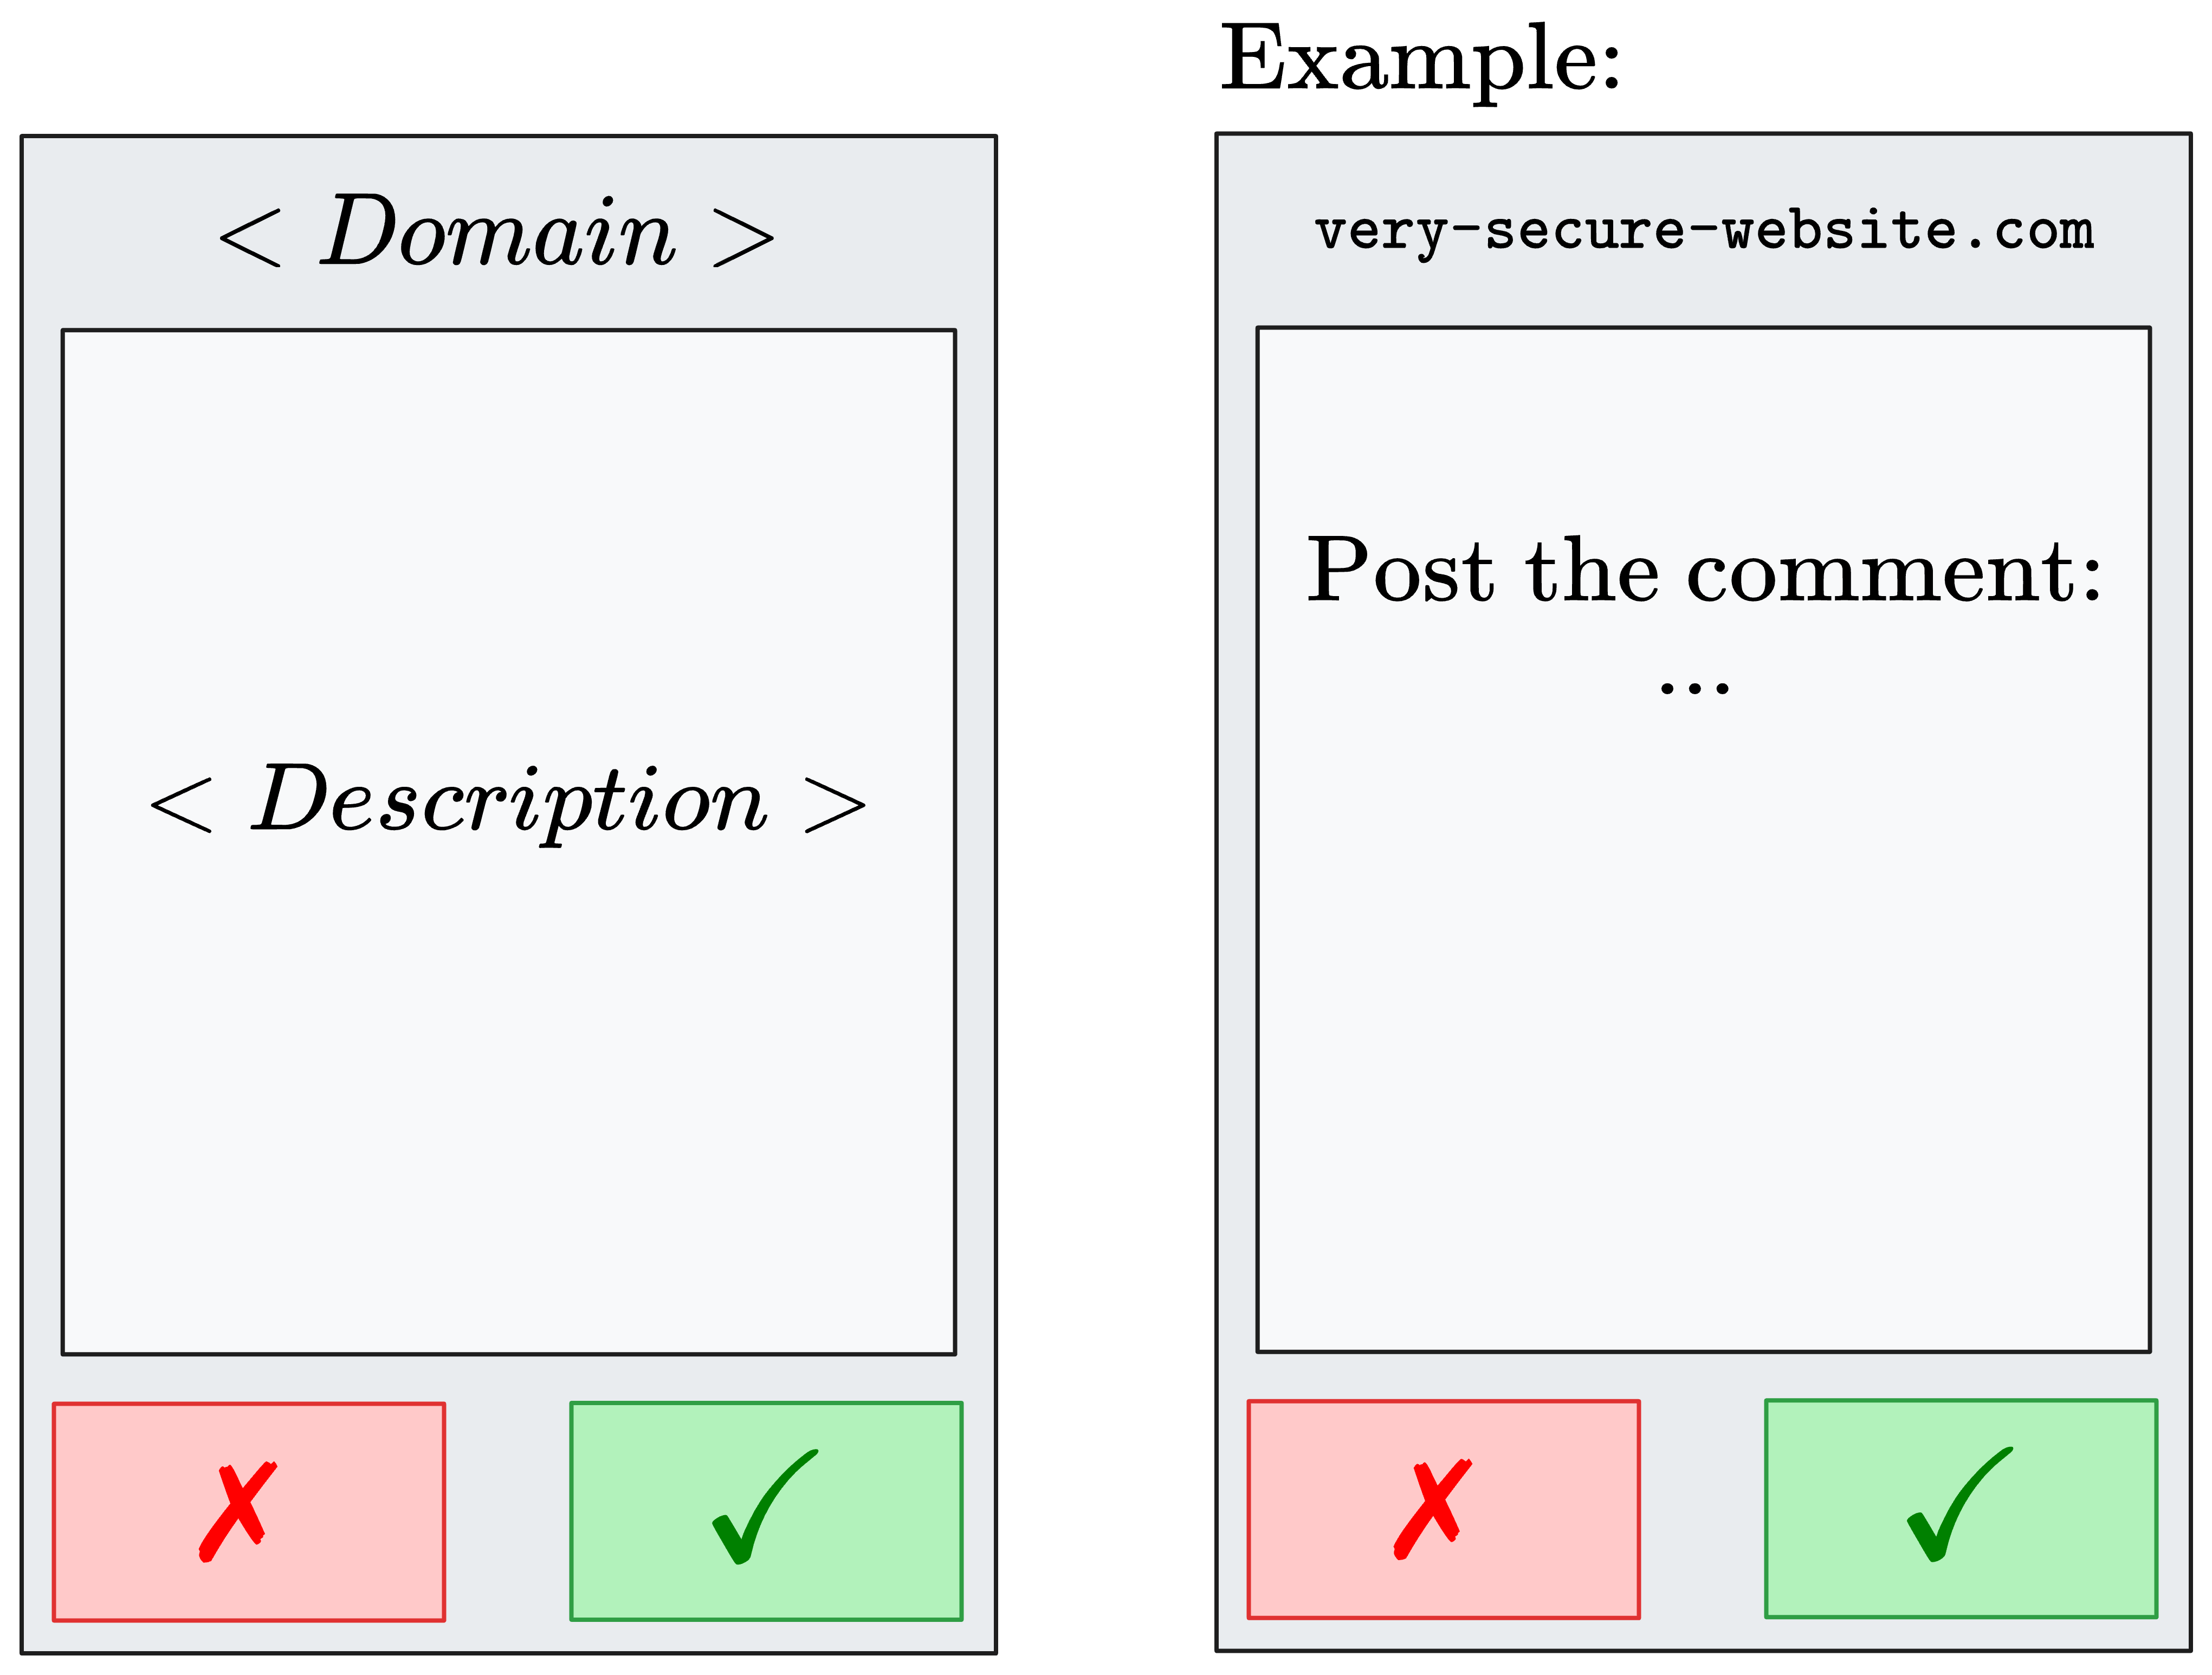
\includegraphics[width=0.5\linewidth]{img/touch-screen-accept-prompt.png}
    \caption{User prompt for accepting or refusing a sensitive request.}
    \label{fig:sensitive-prompt-screen}
\end{figure}
\paragraph{$\boldsymbol{(8)}$}If the user accepts the prompt, query the LR-PUF using the challenge $C_\text{Session}^i$ found within $SensitivePayload$ and the $Domain$ with $query_{BCH}$ to get as a response the error-corrected $seed_i$ before passing it to $KeyGen(seed_i)$ to generate the key pair $(SK_i,PK_i)$.
\paragraph{$\boldsymbol{(9)}$} Sign $SensitivePayload$ with $SK_i$ to prove to the server that the dongle possesses the private key $SK_i$ associated with the currently enrolled session public key $PK_i$.
\paragraph{$\boldsymbol{(10)}$ and $\boldsymbol{(11)}$} $Domain$ and $[SensitivePayload]_{SK_i}$ are sent to the browser. Then the browser sends $[SensitivePayload]_{SK_i}$ as a response to the server to prove ownership of the dongle and user approval of the request. When received, the server will run the function $VerifyDongleSignatureSensitive([SensitivePayload]_{SK_i})$ (Algorithm \ref{alg:verify-dongle-signature-sensitive}).
\begin{algorithm}[ht!]
\caption{$VerifyDongleSignatureSensitive([SensitivePayload]_{SK_i})$}
\begin{algorithmic}[1]
    \Require $[SensitivePayload]_{SK_i}$ and $Cookies$ received from the browser.
    \Ensure  The sensitive request is executed on a valid signature;
             otherwise it is refused.
    \State $V \leftarrow Verify([SensitivePayload]_{SK_i}, SensitivePayload, PK_i)$
    \If{$V = \text{failed}$}
        \State \textbf{return} "Refuse sensitive request"
    \EndIf
    \State $Execute(SensitiveRequest)$
    \State \textbf{return} "Accept sensitive request"
\end{algorithmic}
\label{alg:verify-dongle-signature-sensitive}
\end{algorithm}
\paragraph{$\boldsymbol{\langle12\rangle}$} The server verifies $[SensitivePayload]_{SK_i}$ using $PK_i$.
\paragraph{$\boldsymbol{(13)}$} If the signature is valid, the sensitive request is executed, otherwise, it is refused.

\subsection{Phase 3: Reconfiguration Phase}
The third phase of the protocol described in figure \ref{fig:REPUSH-phase-3} exploits the reconfigurability of the LR-PUF to generate a new key for extending a session. After some time $T_\text{Expiry}$, the session expires and a new key is required in case the user wants to extend the session. Here the following time variables are taken into consideration:
\begin{itemize}
    \item $T_\text{Expiry}$: The maximum session time after which the server requests a session extension by key rotation. Typically $T_\text{Expiry} \gg T_\text{Validity}$. 
    \item $t_\text{start}^{Session}$: Timestamp of when the current session started.
\end{itemize}

\begin{figure}
    \centering
    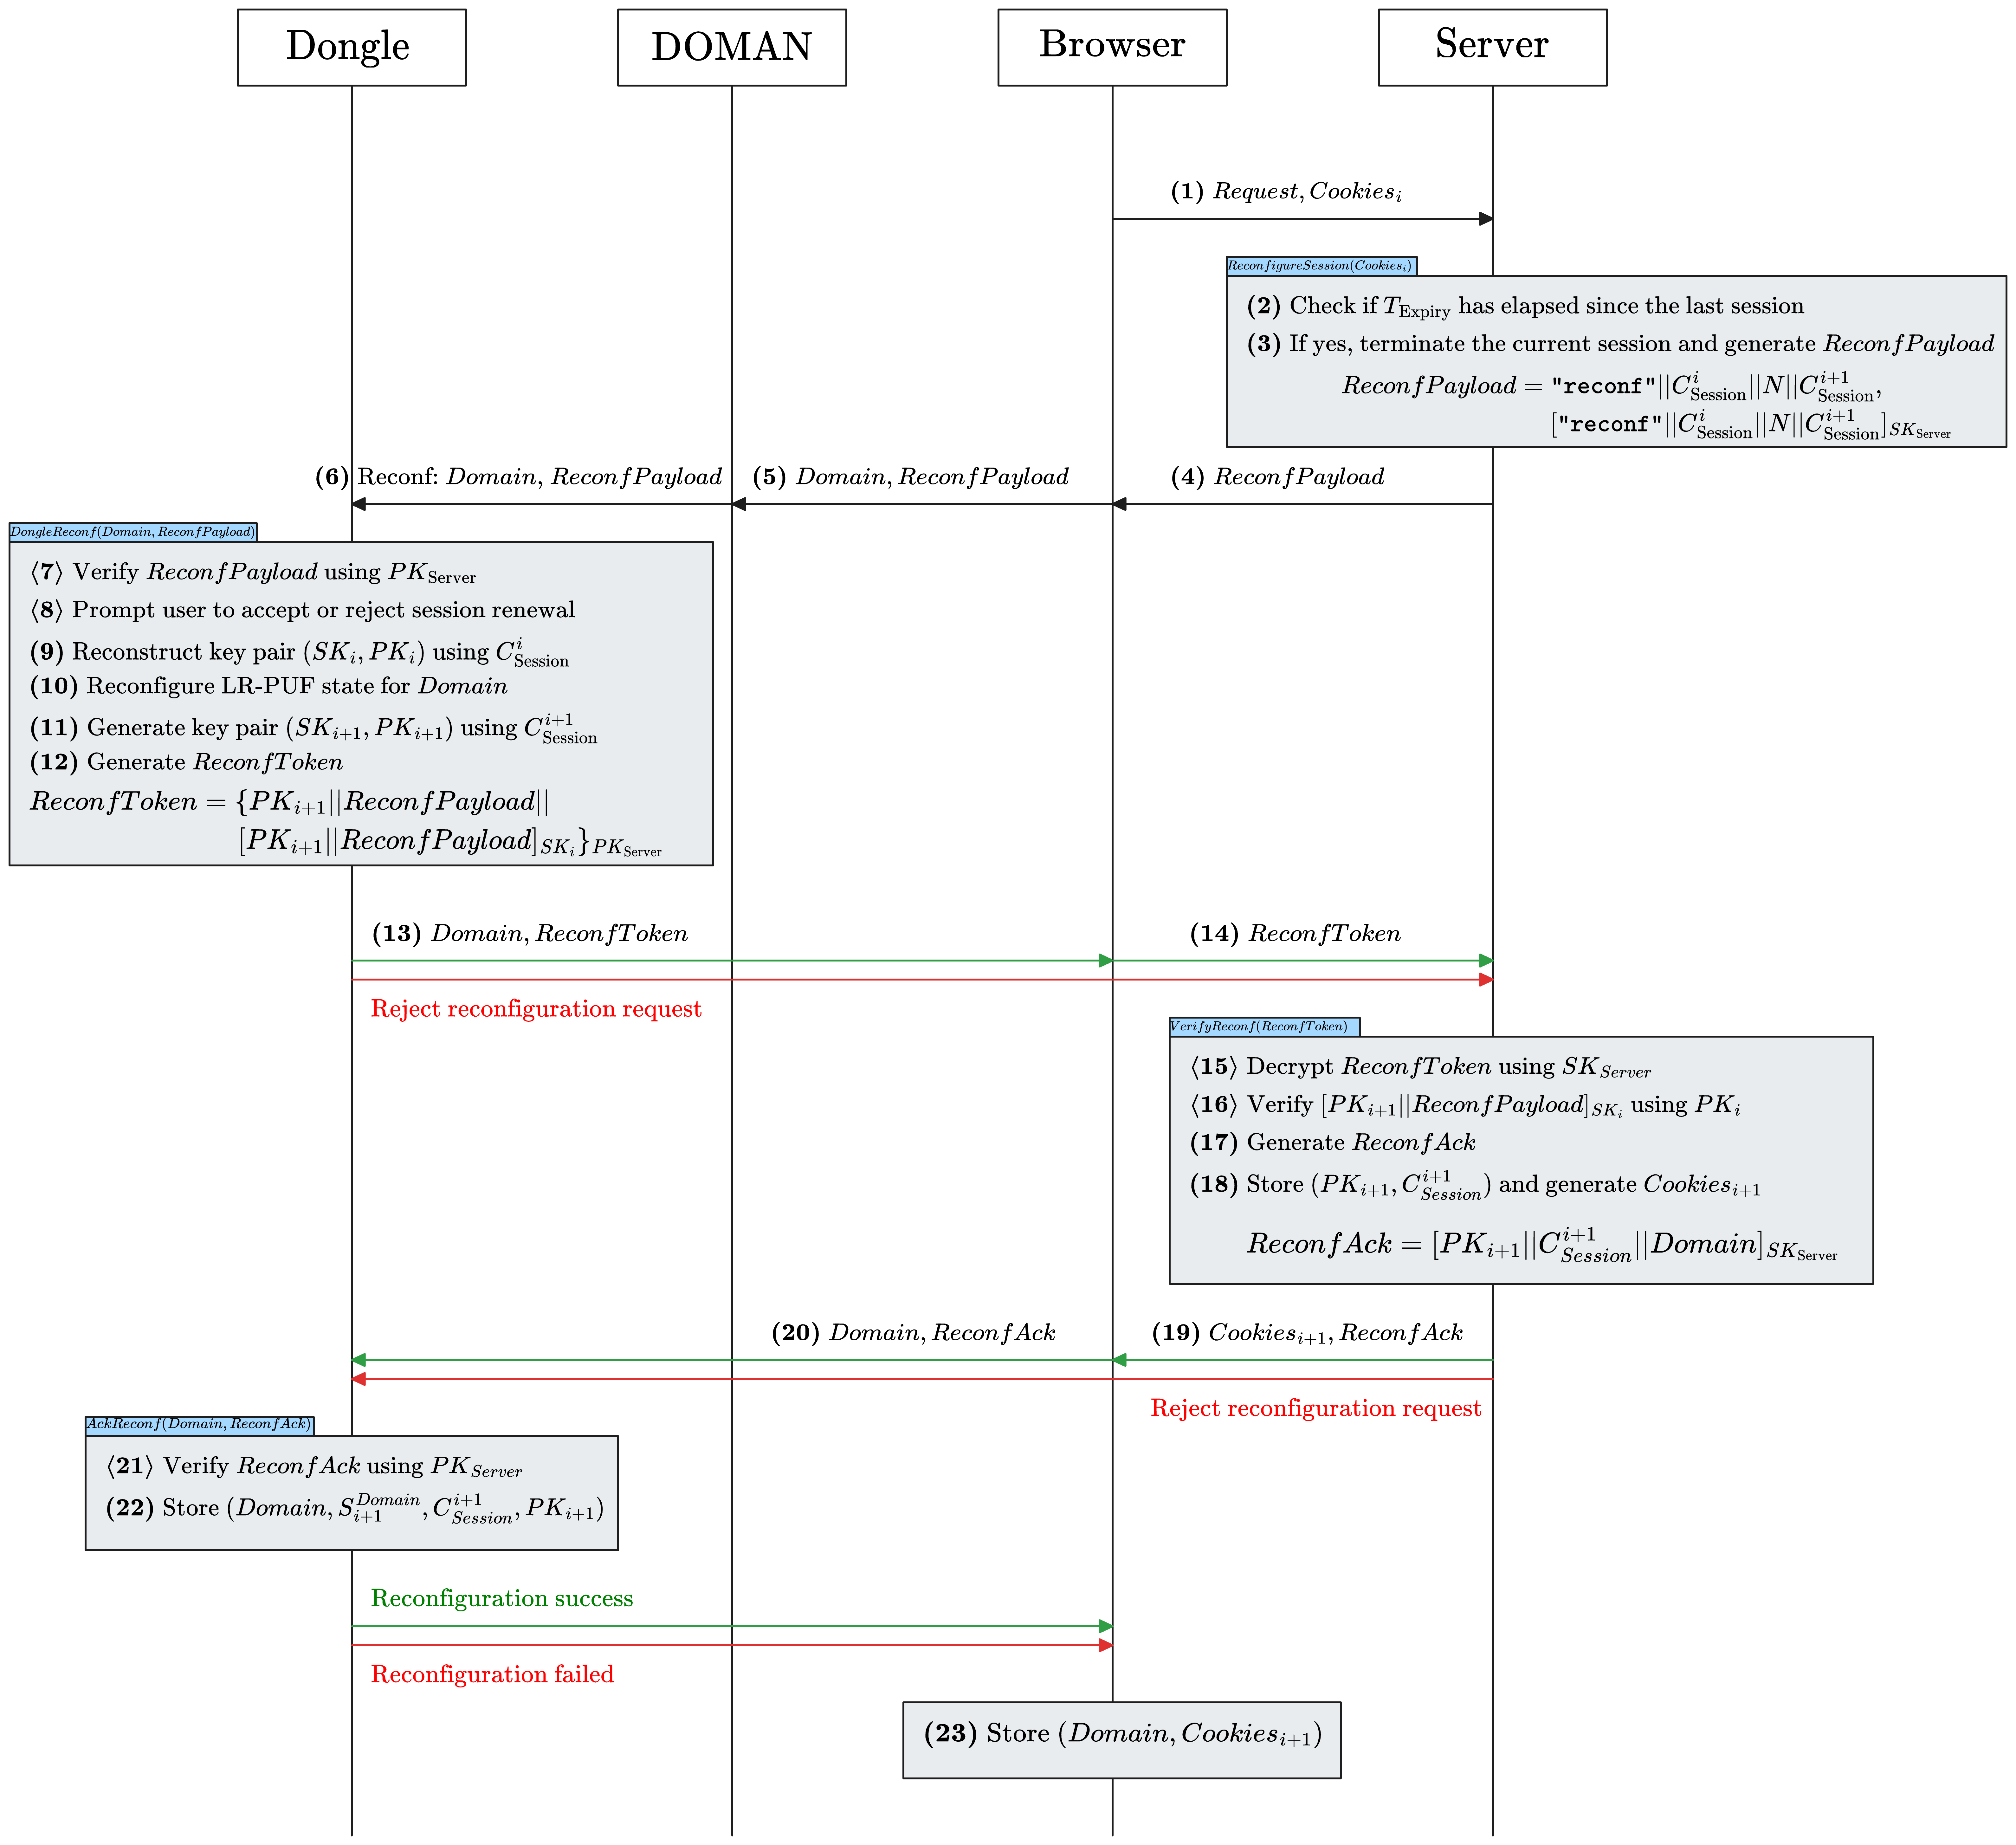
\includegraphics[width=1.2\linewidth]{img/REPUSH-3.png}
    \caption{Phase 3: Reconfiguration Phase}
    \label{fig:REPUSH-phase-3}
\end{figure}

This phase of the protocol is composed of the following steps:
\paragraph{$\boldsymbol{(1)}$} The user makes any request from the browser to the server and presents the current $Cookies_i$. On every received request, the server runs the function $ReconfigureSession(Cookies_i)$ (Algorithm \ref{alg:reconfigure-session}).
\begin{algorithm}[ht!]
\caption{$ReconfigureSession(Cookies_i)$}
\begin{algorithmic}[1]
    \Require Incoming request with $Cookies_i$;
             per-session state including $t^{Session}_{\text{start}}$, $C^i_{\text{Session}}$, and $PK_i$.
    \Ensure  $ReconfPayload$ returned to the browser when the session has expired, otherwise the request is served normally.
    \State $\Delta_\text{Elapsed} \leftarrow Now() - t^{Session}_{\text{start}}$
    \If{$\Delta_\text{Elapsed} < T_{\text{Expiry}}$}
        \State \textbf{return} \texttt{NULL} \Comment{session still within its lifetime}
    \EndIf
    \State $C^i_{\text{Session}} \leftarrow Fetch(Cookies_i)$
    \State $Terminate(Cookies_i)$ \Comment{stop serving requests under the old session}
    \State $N \leftarrow TRNG()$
    \State $C^{i+1}_{\text{Session}} \leftarrow TRNG()$
    \State $m \leftarrow \texttt{"reconf"} || C^i_{\text{Session}} || N || C^{i+1}_{\text{Session}}$
    \State $ReconfPayload \leftarrow (m, [m]_{SK_{\text{Server}}})$
    \State \textbf{return} $ReconfPayload$
\end{algorithmic}
\label{alg:reconfigure-session}
\end{algorithm}
\paragraph{$\boldsymbol{(2)}$} The server checks if $T_\text{Expiry}$ has elapsed since the start of the session to determine if the session has expired or not.
\paragraph{$\boldsymbol{(3)}$} If $T_\text{Expiry}$ has elapsed, then the current session is terminated and we generate $ReconfPayload$ to ask the dongle for a new key:
$$ReconfPayload = (\texttt{"reconf"} || C^i_{\text{Session}} || N || C^{i+1}_{\text{Session}}, [\texttt{"reconf"} || C^i_{\text{Session}} || N || C^{i+1}_{\text{Session}}]_{SK_\text{Server}})$$
\paragraph{$\boldsymbol{(4)}$, $\boldsymbol{(5)}$ and $\boldsymbol{(6)}$} $ReconfPayload$ is sent to the browser. Then the browser sends $Domain$ and $ReconfPayload$ to DOMAN, which then forwards it to the dongle as a reconfiguration request to run the function $DongleReconf(Domain, ReconfPayload)$.
\begin{algorithm}[ht!]
\caption{$DongleReconf(Domain, ReconfPayload)$}
\begin{algorithmic}[1]
    \Require $(Domain, ReconfPayload)$ received from the browser.
    \Ensure  $(Domain, ReconfToken)$ returned to the browser, or an error.
    \State $V_{Payload} \leftarrow Verify(ReconfPayload, PK_{\text{Server}})$
    \If{$V_{Payload} = \text{failed}$}
        \State \textbf{return} "Reject reconfiguration request"
    \EndIf
    \State $\texttt{"reconf"}, C^i_{\text{Session}}, N, C^{i+1}_{\text{Session}} \leftarrow ReconfPayload$
    \State $P \leftarrow UserConfirm(Domain)$
    \If{$P = \text{reject}$}
        \State \textbf{return} "User rejected session renewal"
    \EndIf
%    \State $seed'_i \leftarrow query(C^i_{\text{Session}},Domain)$
%    \State $seed_i \leftarrow ErrorCorrect(seed'_i)$
    \State $seed_i \leftarrow query_{BCH}(Domain, C_\text{Session}^i)$
    \State $SK_i,\ PK_i \leftarrow KeyGen(seed_i)$
%    \State $reconfigure(Domain)$ \Comment{Sets $S^{Domain}_{i+1}$}
%    \State $seed_{i+1} \leftarrow query(C^{i+1}_{\text{Session}},Domain)$
    \State $seed_{i+1} \leftarrow enroll_{BCH}(Domain, C^{i+1}_{\text{Session}},10)$
    \State $SK_{i+1},\ PK_{i+1} \leftarrow KeyGen(seed_{i+1})$
    \State $ReconfToken \leftarrow \{PK_{i+1} || ReconfPayload || [PK_{i+1} || ReconfPayload]_{SK_i}\}_{PK_{\text{Server}}}$
    \State \textbf{return} $(Domain,\ ReconfToken)$
\end{algorithmic}
\label{alg:dongle-reconf}
\end{algorithm}
\paragraph{$\boldsymbol{\langle7\rangle}$} Verify the received $ReconfPayload$ using $PK_\text{Server}$ to make sure that the reconfiguration request is coming from the server.
\paragraph{$\boldsymbol{\langle8\rangle}$} Prompt the user to accept or reject the session renewal or configuration (Figure \ref{fig:sension-renewal-prompt-screen}).
\begin{figure}
    \centering
    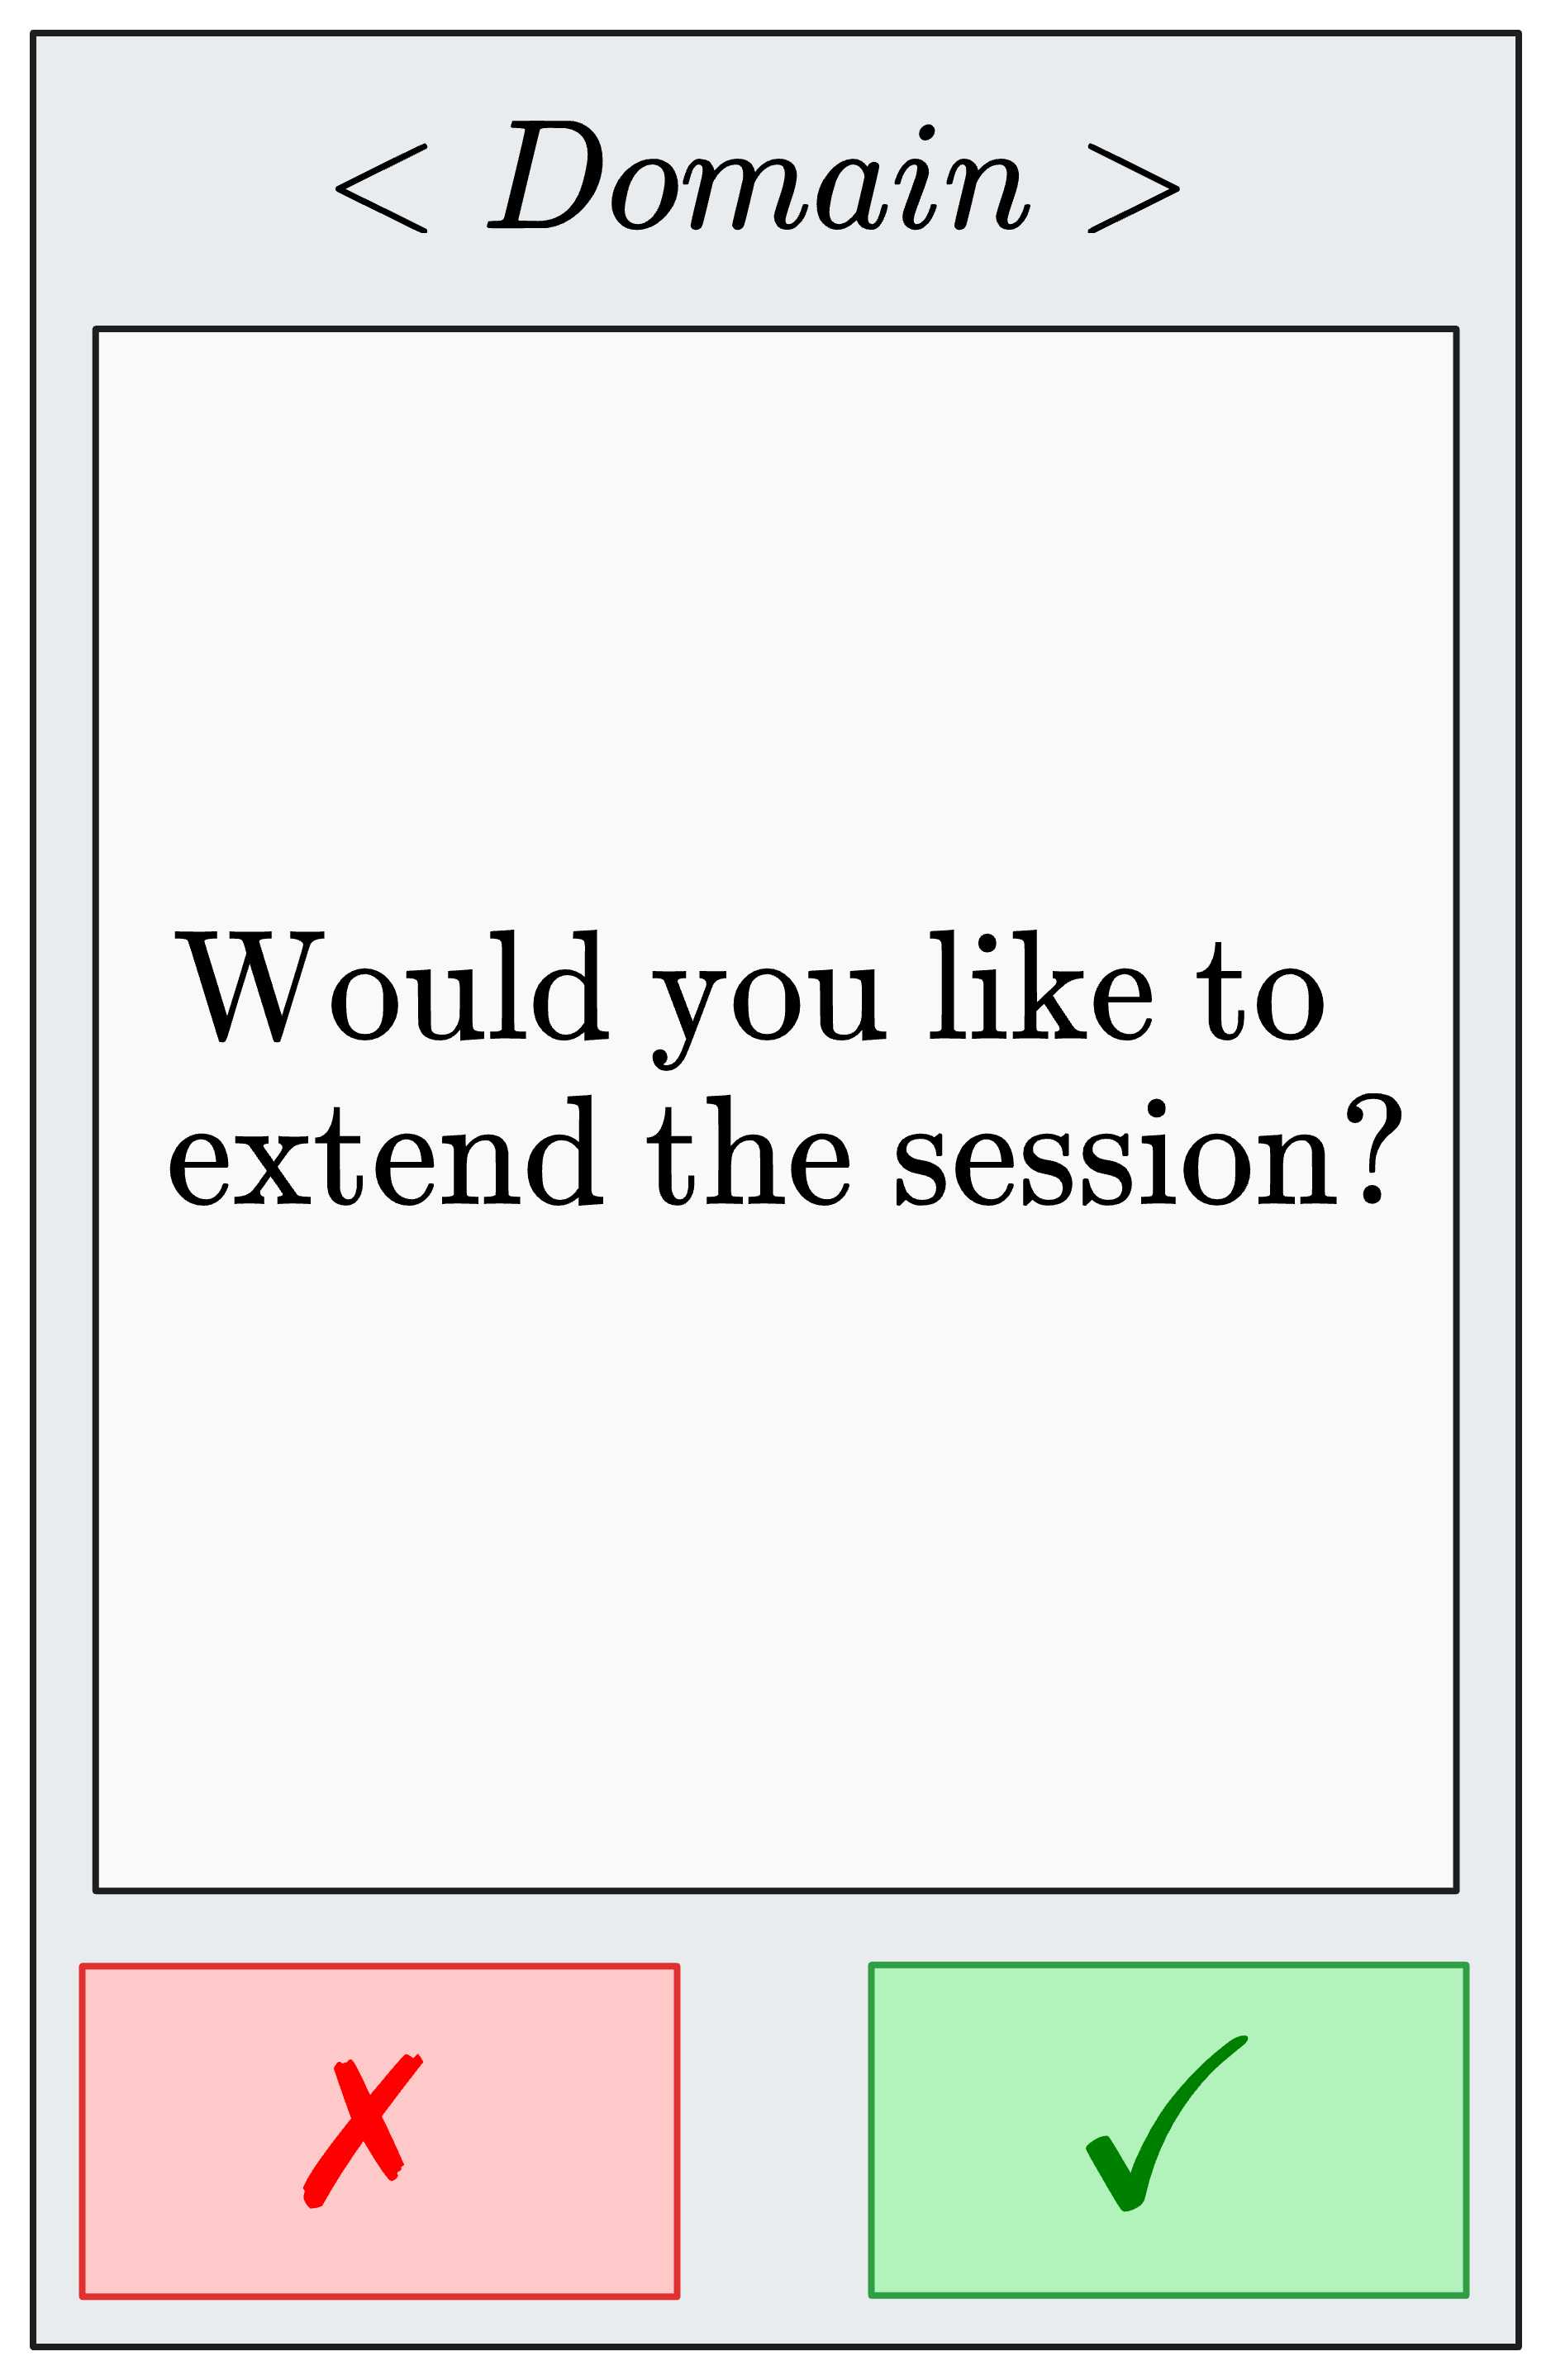
\includegraphics[width=0.3\linewidth]{img/user-prompt-session-renewalp.png}
    \caption{User prompt for session renewal.}
    \label{fig:sension-renewal-prompt-screen}
\end{figure}

\paragraph{$\boldsymbol{(9)}$} If the user accepts the prompt, query the LR-PUF with the $query_{BCH}$ function using the current challenge $C_\text{Session}^i$ found within $ReconfPayload$ and $Domain$ to get the error-corrected $seed_i$ as a response. Then $KeyGen(seed_i)$ is used to generate the key pair $(SK_i,PK_i)$.

\paragraph{$\boldsymbol{(10)}$ and $\boldsymbol{(11)}$} Generate a new key pair for the new session by running $enroll_{BCH}(Domain, C_\text{Session}^{i+1}, 10)$, which will actually run $reconfigure(Domain)$ to get a new state $S_{i+1}^{Domain}$ and then use the new challenge to enroll a new $seed_{i+1}$ which can be error-corrected and then use it to generate the new key pair $(SK_{i+1}, PK_{i+1})$.
\paragraph{$\boldsymbol{(12)}$} $ReconfToken$ is generated as follows to prove to the server that the dongle possesses the current session private key $SK_i$ and then use that to transfer the trust to the new public key $PK_{i+1}$, and the whole token is encrypted with $PK_\text{Server}$ so that only the server can decrypt its contents:
$$ReconfToken = \{PK_{i+1} || ReconfPayload || [PK_{i+1} || ReconfPayload]_{SK_i}\}_{PK_{\text{Server}}}$$
\paragraph{$\boldsymbol{(13)}$ and $\boldsymbol{(14)}$} $Domain$ and $ReconfToken$ are sent to the browser. Then the browser sends $ReconfToken$ as a response to the server. When received, the server runs the function $VerifyReconf(ReconfToken)$ (Algorithm \ref{alg:verify-reconf}).

\begin{algorithm}[ht!]
\caption{$VerifyReconf(ReconfToken)$}
\begin{algorithmic}[1]
    \Require $ReconfToken$ received from the browser.
    \Ensure  $(Cookies_{i+1}, ReconfAck)$ returned to the browser, or an error.
    \State $D \leftarrow Decrypt(ReconfToken, SK_{\text{Server}})$
    \If{$D = \text{failed}$}
        \State \textbf{return} ``Reject reconfiguration request''
    \EndIf
    \State $PK_{i+1},ReconfPayload,[PK_{i+1}||ReconfPayload]_{SK_i} \leftarrow D$
    \State $V \leftarrow Verify([PK_{i+1}||ReconfPayload]_{SK_i}, PK_{i+1}||ReconfPayload, PK_i)$
    \If{$V = \text{failed}$}
        \State \textbf{return} ``Reject reconfiguration request''
    \EndIf
    \State $\texttt{"reconf"}, C^i_{\text{Session}}, N, C^{i+1}_{\text{Session}} \leftarrow ReconfPayload$
    \State $ReconfAck \leftarrow [PK_{i+1}|| C^{i+1}_{\text{Session}}|| Domain]_{SK_{\text{Server}}}$
    \State $store(PK_{i+1},\ C^{i+1}_{\text{Session}})$
    \State $Cookies_{i+1} \leftarrow GenerateCookies()$
    \State $t^{Session}_{\text{last}} \leftarrow Now()$ 
    \State $t^{Session}_{\text{start}} \leftarrow Now()$
    \State \textbf{return} $(Cookies_{i+1}, ReconfAck)$
\end{algorithmic}
\label{alg:verify-reconf}
\end{algorithm}
\paragraph{$\boldsymbol{\langle15\rangle}$} The server decrypts $ReconfToken$ using $SK_\text{Server}$ to get $PK_{i+1}$.
\paragraph{$\boldsymbol{\langle16\rangle}$} $[PK_{i+1}||ReconfPayload]_{SK_i}$ is verified using $PK_i$ to establish that the dongle did produce ${PK_{i+1}}$ and received $ReconfPayload$.
\paragraph{$\boldsymbol{(17)}$} A reconfiguration acknowledgment $ReconfAck$ is generated as follows to prove to the dongle that the server did receive the $ReconfToken$:
$$ReconfAck=[PK_{i+1}|| C^{i+1}_{\text{Session}}|| Domain]_{SK_{\text{Server}}}$$
\paragraph{$\boldsymbol{(18)}$} A new session is created by associating $PK_{i+1}$ with $C^{i+1}_{Session}$ and generating new $Cookies_{i+1}$.
\paragraph{$\boldsymbol{(19)}$} $Cookies_{i+1}$ and $ReconfAck$ are sent to the browser.
\paragraph{$\boldsymbol{(20)}$} $Cookies_{i+1}$ stay in the browser, and $ReconfAck$ and $Domain$ are sent to the dongle for it to run $AckReconf(Domain, ReconfAck)$ (Algorithm \ref{alg:ack-reconf}).
\begin{algorithm}[ht!]
\caption{$AckReconf(Domain, ReconfAck)$}
\begin{algorithmic}[1]
    \Require $(Domain, ReconfAck)$ received from the browser.
    \Ensure  Reconfiguration success and persisted state
             $(Domain, S^{Domain}_{i+1}, C^{i+1}_{\text{Session}}, PK_{i+1})$.
             Otherwise, a reconfiguration error is returned.
    \State $V_{ReconfAck} \leftarrow
            Verify(ReconfAck, PK_{i+1} || C^{i+1}_{\text{Session}} || Domain, PK_{\text{Server}})$
    \If{$V_{ReconfAck} = \text{failed}$}
        \State \textbf{return} ``Reconfiguration not acknowledged''
    \EndIf
    \State $store(Domain, S^{Domain}_{i+1}, C^{i+1}_{\text{Session}},\ PK_{i+1})$
    \State \textbf{return} ``Reconfiguration success''
\end{algorithmic}
\label{alg:ack-reconf}
\end{algorithm}
\paragraph{$\boldsymbol{\langle21\rangle}$} The signature $ReconfAck$ is verified using $PK_{Server}$. If this step fails a reconfiguration error is returned to the browser.
\paragraph{$\boldsymbol{(22)}$} The tuple $(Domain, S_{i+1}^{Domain}, C_{Session}^{i+1}, PK_{i+1})$ is stored on the dongle for it to be used from now on to verify dongle ownership and sign sensitive requests.
\paragraph{$\boldsymbol{(23)}$} On reconfiguration success, $(Domain, Cookies_{i+1})$ is stored on the browser.

By the end of the reconfiguration phase, $PK_{i+1}$ will now be used to verify any signature coming from the dongle. The trust is transferred from $PK_i$ to $PK_{i+1}$. After this the protocol goes back to the second phase until $T_{Expiry}$ is elapsed and a reconfiguration is in order.
